\documentclass[twoside]{article}

\input{settings/packages}
\input{settings/environments}

\definecolor{ugrey}{HTML}{666666}
\definecolor{ured}{rgb}{0.86, 0.08, 0.24}
\definecolor{ured60}{rgb}{0.916, 0.448, 0.544}
\definecolor{ublue}{rgb}{0.12, 0.56, 1.0}
\definecolor{uhole}{rgb}{0.75, 0.75, 0.75}
% \definecolor{ublue}{HTML}{08088A}
% \definecolor{linkcolor}{HTML}{0000CC}
% \definecolor{urlcolor}{HTML}{006600}
% \hypersetup{
%     pdfstartview=FitH,  
%     linkcolor=linkcolor,
%     urlcolor=urlcolor, 
%     colorlinks=true,
%     citecolor=blue}
% базовая подстройка
\renewcommand{\d}{\, d}
\renewcommand{\leq}{\leqslant}
\renewcommand{\geq}{\geqslant}

\newcommand{\vc}[1]{\boldsymbol{#1}}
\newcommand{\1}{\mathbbm{1}}
\newcommand{\T}{^{\textnormal{T}}}
\newcommand{\D}{^{\dag}}
\newcommand{\sub}[2]{#1_{\textnormal{#2}}}
\newcommand{\vp}{\vphantom{\dfrac{1}{2}}}
\newcommand{\hc}{\mathrm{h.c.}}

\renewcommand{\Im}{\mathop{\mathrm{Im}}\nolimits}
\renewcommand{\Re}{\mathop{\mathrm{Re}}\nolimits}
\newcommand{\diag}{\mathop{\mathrm{diag}}\nolimits}
\newcommand{\std}{\mathop{\mathrm{std}}\nolimits}
\newcommand{\mean}{\mathop{\mathrm{mean}}\nolimits}
\newcommand{\sigmoid}{\mathop{\mathrm{sigmoid}}\nolimits}
\newcommand{\card}{\mathop{\mathrm{card}}\nolimits}
\newcommand{\grad}{\mathop{\mathrm{grad}}\nolimits}
\renewcommand{\div}{\mathop{\mathrm{div}}\nolimits}
\newcommand{\rot}{\mathop{\mathrm{rot}}\nolimits}
\newcommand{\Ker}{\mathop{\mathrm{ker}}\nolimits}
\newcommand{\spec}{\mathop{\mathrm{spec}}\nolimits}
\newcommand{\sign}{\mathop{\mathrm{sign}}\nolimits}
\newcommand{\tr}{\mathop{\mathrm{tr}}\nolimits}
\newcommand{\rg}{\mathop{\mathrm{rg}}\nolimits}
\newcommand{\const}{\textnormal{const}}

\newcommand{\grey}[1]{\textcolor{ugrey}{#1}}
\newcommand{\red}[1]{\textcolor{red}{#1}}
\newcommand{\green}[1]{\textcolor{urlcolor}{#1}}
\newcommand{\blue}[1]{\textcolor{ublue}{#1}}

\newcommand{\cmark}{\text{\ding{51}}}
\newcommand{\xmark}{\text{\ding{55}}}

\newcommand{\addletter}[2]{\begin{picture}(7,7) \put(0,#1){{#2)}} \end{picture}}

\newcommand{\ket}[1]{\left| #1 \right\rangle}
\newcommand{\bra}[1]{\left\langle #1 \right|}

\DeclareDocumentCommand{\bk}{m o m}{
    \IfNoValueTF{#2}{\langle #1 | #3 \rangle}{\langle #1 | #2 | #3 \rangle}
}
\newcommand{\kb}[2]{| #1 \rangle \langle #2 |}

\newcommand{\tth}{\sub{t}{th}}
% add page header

% \pagestyle{fancy}
% \fancyhf{}
% \fancyhead[RE,LO]{\thepage}
% \fancyhead[LE,RO]{Ж\raisebox{-1.5pt}{и}К}
% \fancyhead[CO,CE]{\leftmark}
% \fancyfoot[LE,RO]{\thepage}


\input{settings/symbols}

\begin{document}

\input{settings/set}
% !TEX root = ../master-thesis.tex

% document's head

\begin{center}
    % \LARGE \textsc{Fermionic State Preparation and Imaging \\ in Optical Tweezer Array}
    \LARGE \textsc{Tools for 2D Fermi-Hubbard Simulation: \\ State Preparation and Spin-Resolved Imaging}
\end{center}

\hrule

\phantom{42}

\begin{flushright}
    \begin{tabular}{rr}
        % \textbf{Author}: 
        & Khoruzhii Kirill \\
        % & \\
    % date:
        % \textbf{Date}:
        & \textit{Munich, \today}\\
    \end{tabular}
\end{flushright}

\noindent
Quantum simulation with ultracold atoms requires both high-fidelity preparation of the initial many-body state and site-resolved measurement of the final state. This thesis presents the development of experimental techniques for spin-resolved free-space imaging and deterministic, spin-selective preparation of ultracold fermionic $^6$Li atoms in a two-dimensional optical tweezer array. The array is generated using crossed acousto-optic deflectors, with precise control achieved through a combination of direct camera-based calibration and atom-based feedback. A novel spilling method enables the preparation of arbitrary spin- and site-resolved occupation patterns. The thesis also introduces numerical tools for simulating Fermi-Hubbard dynamics in small systems, laying the groundwork for future out-of-equilibrium quantum simulation experiments.







\thispagestyle{empty}

\newpage

\thispagestyle{empty}

\tableofcontents

% \vfill

% Базовая структура диплома:
% \begin{enumerate*}
%     \item deterministic state preparation (single tweezer)
%     \begin{enumerate*}
%         \item loading (2D MOT, MOT, Dipol Trap, Tweezer)
%         \item spilling
%     \end{enumerate*}
%     \item single-atom spin resolved free space imaging
%     \begin{enumerate*}
%         \item ! flashing and model
%         \item ! image processing
%     \end{enumerate*}
%     \item deterministic state preparation (tweezer array)
%     \begin{enumerate*}
%         \item ! generating
%         \item ! control
%         \item ! balancing
%     \end{enumerate*}
% \end{enumerate*}

% Это история про то как сделать и сфотографировать спиновое состояние в твизере.   

% Нужно выписать contributions! И им следовать.   




\newpage



% % !TEX root = ../master-thesis.tex


\section*{Мысли про текст}

Ближайшие шаги:
\begin{enumerate}
	\item Каждая картинка должна быть описана и понятна. 
	\item Описание unirand эксперимента: подробнее про структуру уровней, про картинки.
	\item Вводный рассказ про Fermi Hubbard
	\item Tweezer loading
	\item Tweezer movement
	\item ? MWM
	\item BMF as SAT task
	\item ? Написать про добавки к obj function в линейной модели
	
	% \item Atom based measurements: SVF, , atom-based crosstalk (and comparison)
	
	% \item site- and spin- resolved state preparation

	% \item non-factorizable state preparation, add large Li imgs (see movie)
	 % Можно а-ля the Li добавлять сверху к средним картинкам расшифровку

	% \item Графики для антенн с фитом

\end{enumerate}



\section*{Мысли про figures}


Можно добавить:
\begin{itemize}
	\item ! Схема стабилизации лазеров, какие отстройки, какие частоты, в контексте imaging
	% \item Single atom counting
	\item Демонстрация с Random Unitaries (Xinyi тезис)
	\item Схема установки, фото 3D mot
	% \item BEC
	\item Imaging: разница двух облачков (один, два continous, два alternating)
	% \item Imaging: histogram noise vs atoms, raw nuvu img
	% \item Flashing. Экспериментальная установка, табличка с её параметрами
	% \item State preparation: spilling. Схематичное изображение (посмотреть в Heidelberg thesis).
	% \item ? Экспериментальная последовательность
	\item ? Feshbach resonance
	% \item ? loading issues
	\item ? MWM (simulation, observed)
	\item ? Theory: описание fermi-hubbard, фазовая диаграмма (посмотреть coepsill)
	\item ? Theory: вклад от лабиринтов в локализацию
	% \item ? 2D Step Plot
\end{itemize}



% Huang: 17-25
% Culemann: 15-24




% Sec.\ref{sec:intro} or subsection\ref{subsec:control} Fig.\ref{fig:stepplot} or \eqref{eq:evolution} \newpage


% % !TEX root = ../master-thesis.tex











% \newpage

% \begin{figure}[h]
%     \centering
%     \includegraphics[width=0.5\textwidth]{imgs/tw-setup.jpg}
%     \caption{
%     \textbf{Optical setup for 2D tweezer array.} 
%     The beam path (solid orange line) includes two orthogonal AODs, a $4f$ relay, and diagnostic components. Dashed lines indicate monitoring light paths. Taken from \cite{culemann_construction_2024}.
%     }
%     \label{fig:tw-setup}
% \end{figure}


 












% \begin{figure}
%     \centering
%     \includegraphics{fig-py/imaging-spin-resolved.pdf}
%     \caption{
%         \textbf{Spin-resolved single-atom imaging.}
%         Spatially separated $\sigma_+$ and $\sigma_-$ fluorescence is imaged onto two distinct regions of the camera. The binarization step identifies photon counts above a threshold, followed by a low-pass filter to extract spatially localized signals. Final spin states are assigned based on relative signal strength in each channel:
%         \raisebox{-1pt}{\scalebox{1.5}{\textcolor{ublue}{\textbullet}}} -- $\ket{1}$, 
%         \raisebox{-1pt}{\scalebox{1.5}{\textcolor{ured}{\textbullet}}} -- $\ket{2}$, 
%         \raisebox{-1pt}{\scalebox{1.5}{\textcolor{uhole}{\textbullet}}} -- no atom.
%     }
%     \label{fig:spin-resolved}
% \end{figure}


% Lorem ipsum dolor sit amet, consectetur adipisicing elit, sed do eiusmod
% tempor incididunt ut labore et dolore magna aliqua. Ut enim ad minim veniam,
% quis nostrud exercitation ullamco laboris nisi ut aliquip ex ea commodo
% consequat. Duis aute irure dolor in reprehenderit in voluptate velit esse
% cillum dolore eu fugiat nulla pariatur. Excepteur sint occaecat cupidatat non
% proident, sunt in culpa qui officia deserunt mollit anim id est laborum.


% \newline
% \phantom{42}
% \newline
% \addletter{100}{c} \phantom{4}
% \includegraphics{fig-py/crosstalk-camera-amp.pdf}
% \phantom{4}
% \addletter{100}{d} \phantom{4}
% \includegraphics{fig-py/crosstalk-camera.pdf}
% \hfill
% \phantom{4}

 \newpage


\newpage
% --------------------------------------------------------------------------------------
\section{Introduction} \label{sec:intro}
% --------------------------------------------------------------------------------------
\subsection{The Fermi-Hubbard model}


The simulation of strongly correlated quantum systems remains one of the central challenges in modern physics. While exact numerical methods have provided deep insights in one-dimensional settings, the computational cost of simulating many-body dynamics in higher dimensions grows exponentially with system size, rendering classical approaches impractical. As first envisioned by Feynman, this motivates the development of physical quantum simulators that emulate target Hamiltonians using intrinsically quantum mechanical systems. Among several available platforms, ultracold atoms in optical potentials offer an exceptionally clean and versatile environment for realizing a broad range of many-body models, including the Fermi-Hubbard model relevant for high-temperature superconductivity~\cite{esslinger_fermi-hubbard_2010, gross_quantum_2017}.

In particular, fermionic atoms loaded into optical lattices have enabled the realization of the two-dimensional Fermi-Hubbard model, with site-resolved imaging revealing spin correlations and signatures of antiferromagnetic ordering~\cite{parsons_site-resolved_2016, boll_spin-_2016}. These advances highlight the power of quantum gas microscopy in exploring equilibrium properties of lattice fermions. However, conventional approaches rely on thermal loading of large ensembles into periodic potentials, which often results in uncontrolled entropy and random filling defects. As a consequence, the system is typically initialized in a thermal ensemble, and the preparation of arbitrary low-entropy many-body states remains difficult.

Optical tweezer arrays offer an alternative, bottom-up approach. By providing single-site control, they allow deterministic preparation of initial states, flexible geometries, and site-selective addressing. While initially developed in the context of Rydberg atom arrays~\cite{browaeys_many-body_2020}, these platforms have recently been extended to degenerate fermions, enabling programmable few-body Fermi-Hubbard dynamics~\cite{spar_realization_2022, yan_two-dimensional_2022}. Such results position tweezer arrays as a promising architecture for scalable fermionic quantum simulators.

This thesis contributes to the development of a quantum simulation platform based on ultracold fermionic $^6$Li atoms in a two-dimensional optical tweezer array. In this approach, the array is used for high-fidelity state preparation and control, while the optical lattice serves as the environment for Hamiltonian evolution. Compared to direct loading into a lattice, this separation of initialization and dynamics enables more efficient cooling, deterministic control over occupation patterns, and reduced cycle times. To support this workflow, we develop methods for spin-resolved free-space imaging, arbitrary pattern initialization via spin-selective spilling, and precise tweezer depth balancing.

Looking ahead, such a platform opens the door to nonequilibrium quantum dynamics. For instance, by performing randomized local operations followed by spin-resolved measurements, one can access entanglement entropy via measurement statistics~\cite{brydges_probing_2019}. These protocols offer a practical way to characterize entanglement growth and scrambling, even in regimes where full state tomography is infeasible. Extending such techniques to fermionic systems will provide new insights into thermalization, localization, and quantum information dynamics in strongly correlated matter.

In summary, this work supports the realization of a bottom-up fermionic quantum simulator by combining deterministic state preparation with single-atom, spin-resolved readout. These tools provide a foundation for studying both static and dynamical aspects of the Fermi-Hubbard model in a highly controlled setting.


\subsection{Experimental and computational challenges}
% !TEX root = ../master-thesis.tex

\textbf{Solid-state limitations.} Despite decades of intensive research, fundamental questions about high-temperature superconductivity and many-body localization remain unresolved due to inherent limitations of solid-state systems. Real materials possess complex crystal structures with multiple orbital degrees of freedom, phonon interactions, and intrinsic disorder that obscure the underlying electronic physics \cite{koepsell_quantum_2021}. The limited tunability of material parameters requires synthesizing new compounds for each point in parameter space, making systematic studies of phase diagrams challenging. Furthermore, many key observables remain experimentally inaccessible in solid-state systems. Higher-order spin correlations, real-space magnetic textures, and single-site resolved quantities cannot be directly measured using conventional condensed matter probes, which typically access momentum-space or bulk averaged properties.

\textbf{Computational intractability.} Classical numerical approaches face fundamental obstacles when simulating strongly correlated fermionic systems. The dimension of the Hilbert space grows exponentially with system size, rendering exact diagonalization feasible only for very small clusters. Quantum Monte Carlo methods, while successful for certain bosonic systems, suffer from the fermion sign problem in the presence of frustration or doping, leading to exponentially growing statistical errors \cite{koepsell_quantum_2021}. Approximate methods such as density matrix renormalization group (DMRG) work well in one dimension but become inefficient for two-dimensional systems due to area-law violations in entanglement entropy. These computational limitations severely constrain theoretical understanding of the parameter regimes most relevant to high-temperature superconductivity and many-body localization.

\textbf{Key observables needed.} Progress in understanding both equilibrium and dynamical properties of the Fermi-Hubbard model requires access to observables that are difficult or impossible to measure in conventional systems. For high-temperature superconductivity, key quantities include real-space spin-charge correlations that reveal magnetic polaron formation, site-resolved doping profiles, and the evolution of magnetic correlations with charge carrier density \cite{koepsell_quantum_2021}. For dynamical phase studies, essential observables include local particle densities $\langle n_i(t) \rangle$, magnetization profiles $\langle \sigma^z_i(t) \rangle$, and multi-point correlations that distinguish thermal, Anderson localized, and many-body localized phases. Additionally, investigating dynamical phases requires the ability to prepare arbitrary initial states, control disorder realizations, and perform extensive statistical averaging over many experimental repetitions to extract meaningful signals from noisy quantum dynamics.

\subsection{Ultracold atoms and the tweezer-based approach}
% !TEX root = ../master-thesis.tex

\textbf{Cold atoms advantages.} Ultracold atomic gases provide an exceptionally clean and tunable platform for realizing the Fermi-Hubbard model with unprecedented control over system parameters \cite{esslinger_fermi-hubbard_2010,gross_quantum_2017}. Neutral fermionic atoms such as $^6$Li trapped in optical lattices created by interfering laser beams naturally implement the kinetic energy term through tunneling between neighboring sites. The interaction strength $U$ can be continuously tuned using Feshbach resonances, where an external magnetic field controls the scattering length between atoms in different hyperfine spin states. This allows experimental exploration of the entire phase diagram from the non-interacting limit to strongly correlated regimes. Site-dependent potentials can be introduced using digital micromirror devices or spatial light modulators, enabling controlled studies of disorder effects and many-body localization \cite{choi_exploring_2016,schreiber_observation_2015}.

The development of quantum gas microscopy has revolutionized the field by providing single-site resolution imaging of atomic lattice systems \cite{bakr_quantum_2009,sherson_single-atom-resolved_2010}. These techniques enable direct measurement of local observables such as density correlations, magnetic structure factors, and spin-resolved occupations that are inaccessible in solid-state systems \cite{gross_quantum_2021}. Recent achievements include the observation of antiferromagnetic correlations in two-dimensional Fermi-Hubbard systems \cite{mazurenko_cold-atom_2017,parsons_site-resolved_2016} and demonstrations of many-body localization in disordered lattices \cite{bordia_probing_2017}.

\textbf{Current limitations.} Despite these advances, conventional optical lattice experiments face fundamental constraints in state preparation that limit their potential for studying complex many-body phenomena. Thermal loading from magneto-optical traps produces statistical filling with Poissonian atom number fluctuations, resulting in random defects and uncontrolled entropy that obscure the underlying physics \cite{esslinger_fermi-hubbard_2010}. The harmonic confinement typically present in these systems creates spatial inhomogeneity through varying local chemical potential, leading to "wedding cake" structures with different filling factors across the trap. Additionally, achieving specific initial states required for studying dynamical phases or controlled doping profiles remains challenging with conventional loading methods.

\textbf{Tweezer innovation.} Optical tweezer arrays offer a transformative solution to these state preparation challenges by enabling deterministic, bottom-up assembly of many-body quantum systems \cite{browaeys_many-body_2020}. Individual atoms can be captured and manipulated in tightly focused laser beams, providing single-site control over both spatial and internal degrees of freedom. Recent demonstrations have shown the feasibility of implementing few-body Fermi-Hubbard dynamics in programmable tweezer geometries \cite{spar_realization_2022,yan_two-dimensional_2022}, establishing the foundation for scalable fermionic quantum simulators.

This work advances tweezer-based approaches through the development of crossed acousto-optic deflector (AOD) systems that enable rapid reconfiguration of two-dimensional arrays. The key innovation lies in implementing spin-selective manipulation protocols that allow preparation of arbitrary site- and spin-resolved occupation patterns. Combined with novel imaging techniques for spin-resolved single-shot detection, this platform provides the experimental tools necessary for systematic studies of both equilibrium and dynamical Fermi-Hubbard physics.

\textbf{Separation of preparation and dynamics.} The tweezer-based approach exploits a fundamental insight: optimal state preparation and Hamiltonian evolution can be achieved using different experimental configurations. High-fidelity initial state preparation is performed in the tweezer array, where strong confinement and individual site control enable deterministic loading and spin manipulation. Subsequently, atoms are transferred to an optical lattice optimized for implementing the desired Hamiltonian evolution with precise control over tunneling and interaction parameters. This separation enables access to low-entropy initial states that would be statistically unlikely under thermal loading, opening new possibilities for studying quantum phase transitions, out-of-equilibrium dynamics, and exotic correlated phases.

\subsection{Thesis contributions and outlook}
% !TEX root = ../master-thesis.tex

\textbf{Technical innovations developed.} This work addresses the key experimental bottlenecks limiting progress in Fermi-Hubbard quantum simulation through the development of three interconnected technological advances. The first innovation is a spin-resolved free-space imaging system for $^6$Li atoms that enables simultaneous detection of both hyperfine ground states in a single experimental shot. Unlike previous sequential imaging approaches \cite{bergschneider_spin-resolved_2018}, the implementation utilizes stretched states $|3\rangle$ and $|6\rangle$ with polarization-selective detection paths, achieving \red{99\%} spin discrimination fidelity while maintaining fast imaging times of 20 $\mu$s. This capability provides direct access to local magnetization and spin correlations essential for characterizing magnetic phases and dynamical regimes.

The second major contribution involves the design and control of two-dimensional optical tweezer arrays using crossed acousto-optic deflectors. This work develops calibration protocols that achieve uniform tweezer depths across arrays. A key innovation is the implementation of spin-selective spilling techniques that exploit differential magnetic moments of hyperfine states to enable deterministic preparation of arbitrary site- and spin-resolved occupation patterns. This approach represents the first demonstration of programmable spin-selective state preparation using crossed AOD configurations.

The third component consists of numerical simulation tools that provide theoretical benchmarks for experimental protocols. A custom GPU-accelerated software package was developed that combines exact diagonalization with Krylov subspace methods, enabling simulation of Fermi-Hubbard dynamics in systems up to $10^9$ dimensions. The package supports arbitrary geometries while efficiently computing observables including local densities, spin correlations, and entanglement entropy.

\textbf{Numerical roadmap for dynamical phases.} The computational framework developed in this work serves as both a validation tool for experimental protocols and a roadmap for near-term studies of quantum thermalization and localization. Systematic simulations demonstrate clear signatures that distinguish thermal, Anderson localized, and many-body localized phases through experimentally accessible observables such as imbalance relaxation and entanglement growth. These results provide concrete targets for upcoming experiments and establish the parameter regimes where different dynamical behaviors can be reliably observed with the developed experimental tools.

\textbf{Thesis statement.} This work develops key experimental tools for studying both equilibrium and dynamical aspects of the Fermi-Hubbard model in ultracold atomic systems. By combining deterministic state preparation in programmable tweezer arrays with spin-resolved imaging, the platform enables systematic investigation of magnetic correlations relevant to quantum thermalization phenomena in strongly correlated fermions.

\textbf{Chapter roadmap.} The experimental platform and its capabilities are presented through a sequence of technical developments that build toward the physics applications. Section 2 provides an overview of the overall experimental apparatus. Section 3 details the implementation of spin-resolved free-space imaging, including the optical setup, image processing algorithms, and characterization of detection fidelity. Section 4 describes the tweezer array system, covering AOD control, calibration procedures, and spin-selective state preparation protocols. Section 5 presents the numerical simulation framework and demonstrates its application to studies of dynamical phases in small Fermi-Hubbard systems. Together, these tools establish a foundation for future studies of strongly correlated quantum matter using fermionic systems.

% 
\subsection{Thesis outline}

This thesis describes the development of experimental and computational tools for the preparation and probing of fermionic many-body states in a programmable optical tweezer array. The overarching goal is to enable bottom-up quantum simulation of lattice models, with precise control over initial conditions and single-atom, spin-resolved readout.

Sec.~\ref{sec:imaging} presents the implementation of spin-resolved single-atom imaging of $^6$Li in free space. The section describes the optical layout, the image processing pipeline, and introduces the Su-Schrieffer-Heeger model as a conceptual framework for understanding spin-dependent imaging dynamics.

Sec.~\ref{sec:tweezer} focuses on the creation and control of two-dimensional tweezer arrays. The section begins with the optical setup and AOD control, followed by a detailed discussion of calibration procedures and tweezer depth balancing using both camera-based and atom-based feedback. A key result is the development of a spin-selective spilling technique, enabling the preparation of spin- and site-resolved occupation patterns. Arbitrary configurations are realized through iterative removal steps, formalized via boolean matrix factorization.

Sec.~\ref{sec:mwm} introduces the concept of a matter-wave magnifier—a lensing scheme designed to enhance spatial resolution for future lattice imaging. Although not yet implemented experimentally, fast simulations of wavefunction propagation and Monte Carlo sampling are presented to validate the scheme.

Finally, Sec.~\ref{sec:fhmodel} outlines numerical approaches for simulating Fermi-Hubbard dynamics on small lattices. The computational framework combines exact diagonalization and Krylov-based time evolution, accelerated on GPU hardware. These tools enable simulations of dynamics in the presence of noise and disorder, and serve as a theoretical reference for upcoming experimental investigations.


% Sec.~\ref{sec:appendix} collects supporting material, including technical details of image processing and a description of the Boolean matrix factorization algorithm used for pattern optimization.


\newpage
% --------------------------------------------------------------------------------------
\section{Experimental setup} \label{sec:exp-setup}
% --------------------------------------------------------------------------------------
% !TEX root = ../master-thesis.tex


\begin{figure}[h]
    \centering
    \includegraphics[width=0.33\textwidth]{imgs/setup.png}
    \caption{\red{I will add more text to the image to highlight parts of the system.}}
    \label{fig:setup}
\end{figure}


% !TEX root = ../master-thesis.tex

\begin{figure}[h!]
    \centering
    \addletter{85}{a} \phantom{4}
    \includegraphics[width=1.25in]{imgs/RF.jpg}
    \hspace{1cm}
    \addletter{85}{b} \phantom{4}
    \includegraphics[width=1.25in]{imgs/MW.jpg}
    \caption{
        \textbf{RF and MW antennas used for spin control.}
        (a) PCB-based radiofrequency (RF) antenna used for driving spin transitions at MHz frequencies. 
        (b) Microwave (MW) loop antenna, designed to efficiently couple to hyperfine transitions in $^6$Li. 
        These antennas are used for coherent spin manipulation.
        % performance characterization via spin-flip fidelity is discussed in the following figures.
    }
    \label{fig:rfmw}
\end{figure}


\begin{figure}[h!]
    \centering
    \addletter{130}{a}
    \includegraphics{fig-ai/m-bec-1-joined.pdf}
    \addletter{130}{b}
    \includegraphics{fig-py/m-bec-2.pdf}
    \addletter{130}{c}
    \includegraphics{fig-py/m-bec-3.pdf}
    \caption{
        \textbf{Molecular Bose-Einstein condensate data.}
        (a) Phase space density (PSD) increases as temperature decreases via evaporative cooling, indicating condensation onset. 
        (b) Atom density profiles normalized to unit area; color encodes temperature as in (a).
        (c) At low temperature, the profile shows a bimodal shape: a Gaussian fit to thermal wings (red dots) underestimates the central peak, revealing the mBEC component (blue area).
    }
    \label{fig:mbec}
\end{figure}




\begin{figure}[h!]
    \centering
    \addletter{145}{a}
    \includegraphics{fig-py/atom-counting.pdf}
    \phantom{4242}
    \addletter{145}{b}
    \includegraphics{fig-py/step-plot-2d.pdf}
    \caption{
        (a) Calibration histogram for single-atom counting based on fluorescence signal after after loading to the MOT. Clear quantized peaks correspond to integer atom numbers; the solid red line is a multi-Gaussian fit to the distribution. 
        (b) Measured 2D step plot as a function of tweezer power and magnetic field gradient. Each point indicates the average atom number obtained for a given combination of parameters. This map confirms that for any spill power, a suitable magnetic gradient can be found to achieve a desired quantized atom number.
    }
    \label{fig:spillingadd}
\end{figure}



\newpage
% --------------------------------------------------------------------------------------
\section{Single-atom spin-resolved free-space imaging} \label{sec:imaging}
% --------------------------------------------------------------------------------------

% Motivation and experimental approaches for spin-resolved imaging
\subsection{Introduction} \label{subsec:imaging-motivation} %  of Single-Atom Imaging Techniques
% !TEX root = ../master-thesis.tex




\textbf{Site-resolved and spin-resolved imaging in Fermi-Hubbard physics.}
The experimental realization of strongly correlated quantum systems using ultracold atomic gases in optical lattices has become a versatile platform for quantum simulation \cite{esslinger_fermi-hubbard_2010,gross_quantum_2017}. The Fermi-Hubbard model provides a framework for understanding high-temperature ,superconductivity, quantum magnetism, and exotic phases of matter. However, extracting meaningful information about complex phenomena in these systems requires detection techniques that can probe the system at the microscopic level.

Single-site resolution is essential for studying physics in optical lattices. Traditional detection methods measure only integrated quantities such as total particle number or momentum distribution, providing limited insight into spatial correlations and local properties \cite{gross_quantum_2021}. Quantum gas microscopy enables direct observation of individual atoms at specific lattice sites \cite{bakr_quantum_2009,sherson_single-atom-resolved_2010}. This capability has proven valuable for measuring key observables in correlated systems, including density-density correlations, charge fluctuations, and the characterization of different phases.

Beyond spatial resolution, the detection of internal atomic degrees of freedom, particularly spin states, provides access to additional physics. In fermionic systems, spin governs exchange interactions, Pauli exclusion effects, and magnetic ordering phenomena \cite{parsons_site-resolved_2016,boll_spin-_2016}. The ability to distinguish between different spin states enables direct measurement of spin correlations, antiferromagnetic ordering, and other magnetic phenomena that emerge from the interplay between kinetic energy, interaction strength, and filling factor.

The combination of site-resolved and spin-resolved detection capabilities represents an important development in quantum gas microscopy. This approach enables simultaneous measurement of both spatial and spin degrees of freedom, providing access to the full wavefunction structure \cite{mazurenko_cold-atom_2017}. Such measurements have revealed phenomena including the emergence of antiferromagnetic correlations in doped Mott insulators, the formation of magnetic polarons, and spin-charge separation effects. Recent experimental achievements have demonstrated this approach through direct visualization of stripe formation in mixed-dimensional systems \cite{bourgund_formation_2025} and the characterization of entanglement structures through position and momentum correlations \cite{bergschneider_experimental_2019}.

The importance of combined site and spin resolution extends beyond fundamental studies to applications in quantum simulation and quantum information processing. Phenomena such as spin liquids, topological phases, and unconventional superconducting states exhibit signatures that are accessible through simultaneous measurement of spatial and spin correlations. As detailed in Section 5, the experimental investigation of localization phenomena presents additional motivation for advanced imaging capabilities. The characterization of localized phases, thermalization dynamics, and the transition between localized and thermal behavior requires access to local observables and their correlations across different length scales. Combined site and spin resolution provides the necessary tools to probe these phenomena directly, enabling studies of local magnetization patterns, spin transport, and the breakdown of thermalization in disordered quantum systems.

The technical challenges associated with implementing simultaneous site and spin resolution have driven innovation in experimental techniques. Traditional approaches often require sequential measurements or complex state preparation protocols that can introduce systematic errors or limit measurement fidelity. The development of efficient, simultaneous detection schemes represents a step toward realizing the potential of quantum gas microscopy platforms for studying correlated quantum matter.


% ----------------------------------------------------------------------------------------------------------------------------------------------------------------------------------------------------------------------
% ----------------------------------------------------------------------------------------------------------------------------------------------------------------------------------------------------------------------
% ----------------------------------------------------------------------------------------------------------------------------------------------------------------------------------------------------------------------

\textbf{Quantum gas microscopy with Raman sideband cooling.}
The foundation of modern quantum gas microscopy relies on fluorescence imaging of individual atoms trapped in optical lattices. Early implementations achieved single-site resolution through direct fluorescence detection, where atoms scattered resonant photons that were collected by high numerical aperture objectives \cite{bakr_quantum_2009,sherson_single-atom-resolved_2010}. However, this approach faced fundamental limitations due to the heating effects of scattered photons and the finite lifetime of excited atomic states, which limited the achievable signal-to-noise ratio and detection fidelity.

The introduction of Raman sideband cooling during the imaging process addressed these fundamental limitations and enabled high-fidelity detection of fermionic atoms \cite{lester_raman_2014,cheuk_quantum-gas_2015,preiss_quantum_2015}. In this approach, atoms are simultaneously cooled to their motional ground state while being imaged, allowing for extended interaction times with the imaging light without significant heating or loss. The Raman cooling process involves two laser fields: a cooling beam that drives transitions from excited motional states to lower motional states, and an imaging beam that provides the fluorescence signal for detection.

The cooling mechanism operates through stimulated Raman transitions that couple different motional states of the trapped atom. When an atom absorbs a photon from the imaging beam and subsequently emits a photon into the cooling beam mode, the energy difference corresponds to the motional quantum, effectively removing vibrational energy from the atom. This process continues throughout the imaging sequence, maintaining the atom close to the motional ground state and preventing escape from the trapping potential.

Several technical requirements must be satisfied for effective Raman cooling imaging. The frequency detuning between the cooling and imaging beams must match the trap frequency to ensure resonant coupling between motional states. The intensity and polarization of both beams require careful optimization to achieve efficient cooling while maintaining sufficient fluorescence for detection. Additionally, the spatial overlap between the cooling and imaging beam modes must be precisely controlled to ensure uniform cooling across the entire imaging region.

The advantages of Raman cooling imaging for site-resolved detection are substantial. Extended imaging times, typically lasting several milliseconds, allow for the collection of thousands of photons per atom, resulting in high signal-to-noise ratios and detection fidelities exceeding 99\% \cite{cheuk_quantum-gas_2015}. The continuous cooling during imaging prevents atoms from heating out of the imaging focus, maintaining sharp, well-defined atomic images throughout the detection sequence. This capability is particularly important for fermionic atoms, where Pauli exclusion prevents the use of sub-Doppler cooling techniques that are available for bosonic species.

% Recent developments have focused on optimizing the speed and efficiency of Raman cooling imaging protocols through improvements in laser stabilization, beam shaping, and detection optics. These advances have enabled more robust and reliable imaging systems while maintaining the high detection fidelities required for precision measurements in quantum many-body systems.

Despite these advances, Raman cooling imaging presents several technical challenges. The requirement for precise frequency control of multiple laser systems increases experimental complexity. The cooling efficiency depends critically on the trap depth and geometry, requiring careful optimization for different experimental configurations. Furthermore, the imaging process itself can introduce systematic effects, such as light shifts or unwanted state preparation, that must be carefully characterized and controlled.

The integration of additional detection capabilities, such as spin resolution, into existing Raman cooling imaging setups presents both opportunities and challenges. The existing laser systems and detection optics provide a foundation for implementing spin-selective imaging schemes, but additional complexity is required to distinguish between different internal atomic states while maintaining the cooling and imaging functionality.


% ----------------------------------------------------------------------------------------------------------------------------------------------------------------------------------------------------------------------
% ----------------------------------------------------------------------------------------------------------------------------------------------------------------------------------------------------------------------
% ----------------------------------------------------------------------------------------------------------------------------------------------------------------------------------------------------------------------

\textbf{Spin-resolved detection for Raman imaging.}
The extension of quantum gas microscopy to include spin resolution represents a significant technical challenge, particularly when integrated with Raman sideband cooling protocols. While Raman cooling imaging provides excellent spatial resolution and detection fidelity, the addition of spin selectivity requires careful consideration of how different internal atomic states interact with the imaging and cooling light fields. Several approaches have been developed to achieve spin-resolved detection while maintaining the advantages of Raman cooling.

Sequential imaging approaches represent the most straightforward method for achieving spin resolution in lattice-based systems. In this scheme, atoms in different spin states are imaged in separate experimental cycles, with state-specific preparation or selection applied before each imaging sequence \cite{boll_spin-_2016,parsons_site-resolved_2016}. For example, one can first image all atoms, then apply a spin-selective removal pulse to eliminate one spin component, and image again to determine the distribution of the remaining spin state. The primary advantage of sequential imaging lies in its compatibility with existing Raman cooling infrastructure, requiring no modifications to imaging optics or laser systems while preserving full detection fidelity for each spin component. However, sequential imaging suffers from fundamental limitations: the requirement for multiple experimental cycles significantly reduces data acquisition rates, shot-to-shot fluctuations introduce additional noise sources, and most importantly, sequential detection cannot access simultaneous correlations between different spin states, limiting its applicability to studies of magnetic ordering and spin dynamics.

Stern-Gerlach separation techniques offer an alternative approach that can provide simultaneous spin detection. In this method, atoms are released from the optical lattice and subjected to a magnetic field gradient that spatially separates different spin states based on their magnetic moments. Early implementations of this approach focused on one-dimensional systems or utilized the separation to divide the atomic cloud into distinct regions for subsequent analysis \cite{boll_spin_2016}. More sophisticated developments have emerged, which combines an initial Stern-Gerlach splitting into adjacent layers of a highly stable vertical superlattice with subsequent charge pumping to separate the layers, enabling independent high-resolution images of each layer \cite{koepsell_robust_2020}.

% The integration challenges for spin-resolved detection with Raman cooling extend beyond the specific detection schemes to include fundamental considerations about state preparation and measurement protocols. The cooling light fields can induce unwanted optical pumping between different internal states, potentially compromising spin resolution. The requirement for precise control of polarization, magnetic fields, and laser frequencies increases the overall system complexity and introduces additional sources of technical noise. Furthermore, the measurement process itself can introduce correlations between nominally independent degrees of freedom. For example, the efficiency of Raman cooling may depend on the internal state of the atom, leading to state-dependent detection fidelities that must be carefully characterized and corrected. Similarly, light shifts induced by the imaging beams can modify the internal state structure, affecting the selectivity of spin-dependent processes.

While the approach demonstrated in \cite{koepsell_robust_2020} represents perhaps the most advanced spin-resolved detection scheme for lattice systems to date, its implementation complexity is substantial. The technique requires precise integration of Stern-Gerlach separation, charge pumping protocols, and careful optimization of the optical imaging path to prevent interference between light scattered from different layers. 
% The need for stable vertical superlattices and accurate control of interlayer separations presents additional technical challenges that limit the broader adoption of this approach.



% ----------------------------------------------------------------------------------------------------------------------------------------------------------------------------------------------------------------------
% ----------------------------------------------------------------------------------------------------------------------------------------------------------------------------------------------------------------------
% ----------------------------------------------------------------------------------------------------------------------------------------------------------------------------------------------------------------------


\textbf{Free-space imaging.} Free-space fluorescence imaging represents an alternative approach to traditional Raman-cooled quantum gas microscopy, where atoms are imaged without confining potentials during the detection process. This paradigm eliminates the technical complexity of maintaining tight trapping and cooling during imaging, potentially enabling faster detection protocols and simplified experimental setups.

The Heidelberg group demonstrated pioneering work in spin-resolved free-space imaging of fermionic $^6$Li atoms \cite{bergschneider_spin-resolved_2018}. Their approach achieved single-atom detection fidelities of up to 99.4(3)\% by collecting approximately 20 fluorescence photons per atom during a 20 $\mu$s exposure. To mitigate acceleration from radiation pressure, they employed two counter-propagating laser beams with alternating 200 ns pulse sequences. Spin resolution was implemented through sequential imaging schemes, where different hyperfine states were addressed in successive exposures by shifting laser frequencies. While this sequential approach enabled spin-selective detection, it inherently limited access to simultaneous spin-spin correlations. Recent developments by the Greiner group have significantly advanced the speed and efficiency of free-space detection protocols \cite{su_fast_2025}. Their implementation achieved detection times as short as 2.4 $\mu$s while maintaining high detection fidelities. The demonstrated capability for parity-projection-free imaging represents a significant advantage, enabling direct counting of multiple atoms per site without light-assisted collisions.

For experiments requiring small lattice spacings, matter-wave magnification (MWM) has emerged as a crucial enabling technology \cite{murthy_matter-wave_2014, asteria_quantum_2021}. MWM techniques coherently expand atomic distributions before detection, circumventing diffraction-limited resolution while preserving site-resolved capability. By adiabatically manipulating harmonic potentials, spatial patterns can be magnified by factors of 10-50, enabling free-space imaging of systems with sub-micrometer lattice spacings.

The technical implementation of free-space imaging requires optimization of competing factors: imaging duration must be minimized to prevent significant atomic motion due to photon recoil, while collecting sufficient photons for reliable detection. For $^6$Li atoms, the relatively large recoil energy leads to position spreads of approximately 10 $\mu$m during typical imaging times. Performance trade-offs between free-space and lattice-based approaches depend on experimental priorities: free-space imaging offers superior detection speed, reduced complexity and simultaneous multi-component detection capabilities, while lattice-based methods typically provide better spatial resolution.


\textbf{This work.} This work implements spin-resolved free-space imaging for $^6$Li atoms using simultaneous detection of stretched states $|3\rangle$ and $|6\rangle$ with polarization-selective optics. Atoms are transferred to these stretched states, which exhibit nearly pure $m_J = \pm 1/2$ character at high magnetic fields and couple strongly to $\sigma^{\pm}$ polarized light. A polarizing beam splitter after the imaging objective spatially separates the $\sigma^+$ and $\sigma^-$ fluorescence components onto distinct regions of the camera.

The implementation achieves 99\% spin discrimination fidelity while maintaining imaging times of 20 $\mu$s. Compared to previous approaches \cite{bergschneider_spin-resolved_2018}, which required sequential imaging cycles within a single experimental shot, our single-exposure detection simplifies the experimental sequence.
 % and reduces sensitivity to technical fluctuations. While the fundamental capabilities are similar, the streamlined approach facilitates integration with the rapid experimental cycles necessary for high-statistics studies of quantum dynamics.

The technique provides access to spin-dependent observables including local magnetization $\langle \sigma^z_i \rangle$ and spin correlations, essential for characterizing magnetic phenomena in Fermi-Hubbard systems. 
% The fast imaging protocol is designed for compatibility with the deterministic state preparation capabilities described in Section 4, enabling systematic studies of many-body dynamics with precisely controlled initial conditions.
Future integration with optical lattice system and MWM will enable
% transfer of deterministically prepared atomic configurations for 
investigation of dynamical phases including quantum thermalization, Anderson localization, and many-body localization. 
% Combined with the numerical simulation framework presented in Section 5, 
% This platform provides tools for systematic exploration of strongly correlated quantum matter in controllable fermionic systems.

\subsection{\texorpdfstring{$^6$Li}{6Li} hyperfine structure and imaging scheme} \label{subsec:imaging-hyperfine}
% !TEX root = ../master-thesis.tex





\begin{figure}
    \centering
    \addletter{200}{a}
    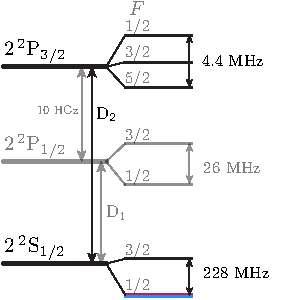
\includegraphics{fig-ai/li-levels-base.pdf}
    \hspace{1cm}
    \addletter{200}{b}
    \includegraphics{fig-ai/li6-zeeman-broken-ai.pdf}
    \caption[${}^6$Li energy levels]{
        \textbf{${}^6$Li energy levels}. 
        a) Level diagram of the ground and excited states of ${}^6$Li \cite{gehm_preparation_2003}, including the D1 and D2 transitions around $\lambda = 671$~nm. 
        b) Zeeman splitting of the hyperfine levels of the $2\, {}^2\mathrm{S}_{1/2}$ and $2\, {}^2\mathrm{P}_{2/2}$ in ${}^6$Li \cite{serwane_deterministic_2011, sibalic_arc_2017}. As different spin states for physics we consider state $\ket{1}$ and $\ket{2}$, but for imaging it is worth to flip them to stretched states $\ket{6}$, $\ket{3}$. Colored lines indicate transitions driven by radiofrequency (RF) and microwave (MW) fields.
    }
    \label{fig:li6levels}
\end{figure}


% \subsection{$^6$Li hyperfine structure and imaging scheme}

The $^6$Li atom possesses a relatively simple electronic structure that makes it well-suited for quantum gas experiments. The electronic ground state $2\,^2\mathrm{S}_{1/2}$ exhibits hyperfine splitting due to the interaction between the electron and nuclear spins, resulting in two manifolds with total angular momentum $F = 1/2$ and $F = 3/2$ separated by 228 MHz (Fig.~\ref{fig:li6levels}a). The excited $2\,^2\mathrm{P}$ states relevant for optical transitions around $\lambda = 671$ nm include both the $\mathrm{P}_{1/2}$ (D$_1$ line) and $\mathrm{P}_{3/2}$ (D$_2$ line) levels \cite{gehm_preparation_2003}.

For quantum simulation experiments, the two lowest hyperfine states $|F = 1/2, m_F = \pm 1/2\rangle$, commonly denoted as $|1\rangle$ and $|2\rangle$, serve as the effective spin-1/2 system for realizing the Fermi-Hubbard model. These states exhibit favorable scattering properties and can be brought into resonant interaction using Feshbach resonances near accessible magnetic field strengths.

However, for fluorescence imaging, the stretched states $|3\rangle$ and $|6\rangle$ offer significant advantages over the $|1\rangle$ and $|2\rangle$ states. As shown in Fig.~\ref{fig:li6levels}b, at magnetic fields above $\sim 100$ G, the stretched states acquire nearly pure $m_J = \pm 1/2$ character due to Zeeman splitting \cite{serwane_deterministic_2011, sibalic_arc_2017}. This results in strong coupling to circularly polarized light: state $|3\rangle$ couples primarily to $\sigma^-$ transitions while $|6\rangle$ couples to $\sigma^+$ transitions. The stretched nature ensures closed cycling transitions with minimal population leakage to other hyperfine states, enabling efficient photon scattering rates exceeding those achievable with $|1\rangle$ and $|2\rangle$.

The imaging protocol therefore involves a preliminary step where atoms are transferred from the $|1\rangle$ and $|2\rangle$ physics states to the $|3\rangle$ and $|6\rangle$ imaging states using radiofrequency or microwave pulses. The polarization selectivity of the stretched states then enables spatial separation of the fluorescence signals using polarizing optics, as detailed in Section 3.4. This approach preserves the spin information while optimizing detection efficiency through the enhanced scattering cross-sections of the stretched states.

\subsection{Su-Schrieffer-Heeger model} \label{subsec:imaging-ssh}
% !TEX root = ../master-thesis.tex



\begin{figure}
    \centering
    \addletter{140}{a}
    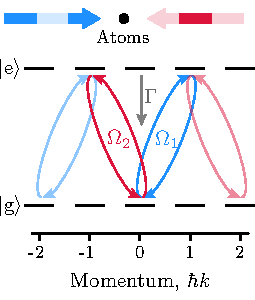
\includegraphics{fig-ai/ssh-scheme.pdf}
    \hfill
    \addletter{140}{b}
    \includegraphics{fig-py/ssh-model.pdf}
    \caption[Numerical simulation of momentum-space dynamics in the SSH model]{
        \textbf{Numerical simulation of momentum-space dynamics in the SSH model}. 
        a) Atoms undergo momentum-changing transitions via couplings $\Omega_1$ and $\Omega_2$, realizing a SSH-like quantum walk.
        b) Momentum distributions over time for different beam configurations: single beam (left) shows small shift; two continuous beams (middle) result in fast spreading; alternating beams (right) suppress spread.
    }
    \label{fig:sshmodel}
\end{figure}


Understanding the fundamental limitations and optimal strategies for free-space imaging requires a theoretical framework that captures the interplay between photon scattering, momentum transfer, and spatial resolution. This section develops a model based on the Su-Schrieffer-Heeger (SSH) Hamiltonian to explain the motivation for alternating beam sequences and to estimate the characteristic resolution limits of the imaging scheme.



% \textbf{Recoil heating and momentum diffusion.} 
Although $^6$Li is a light atom and experiences relatively large momentum recoil during scattering, its broad D2 transition at $\lambda = 671$ nm allows for rapid photon emission. The typical recoil velocity is given by $v_\mathrm{rec} = h/(m\lambda)$, where $m$ is the atomic mass of $^6$Li and $\lambda$ is the wavelength of the imaging light. As the atom scatters photons at a rate $\Gamma$, each with random emission direction, it undergoes a random walk in momentum space, resulting in spatial diffusion during the imaging pulse.

The root-mean-square width of this random walk is approximately \cite{kruip_design_2024}
\begin{equation}
\sigma_\mathrm{rw} = \frac{1}{3} v_\mathrm{rec} \Gamma^{1/2} t^{3/2},
\label{eq:sigmarw}
\end{equation}
where $t$ is the total exposure time. For a fixed number of scattered photons $N_\mathrm{ph}$, we can express $t = N_\mathrm{ph}/\Gamma$, yielding
\begin{equation}
\sigma_\mathrm{rw} = \frac{1}{3} v_\mathrm{rec} \Gamma^{-1} N_\mathrm{ph}^{3/2}.
\end{equation}
This scaling highlights the trade-off between collecting more fluorescence photons and maintaining spatial resolution. In our system, with $N_\mathrm{ph} \approx 300$ scattered photons (of which approximately 10\% are detected by the camera), the resulting diffusion is on the scale of 11 $\mu$m, which sets the practical limit for spatial resolution in free-space imaging of $^6$Li atoms.


% \textbf{SSH model.} 
The scattering dynamics of a freely moving atom illuminated by resonant counter-propagating beams can be understood as a momentum-space quantum walk that maps onto the Su-Schrieffer-Heeger (SSH) model. In the standard SSH model, particles hop between two sublattices with alternating coupling strengths:
\begin{equation}
H = t_1 \sum_n |n,B\rangle \langle n,A| + t_2 \sum_n |n+1,A\rangle \langle n,B| + \text{h.c.}
\end{equation}
For the atomic case, this model takes the form:
\begin{equation}
H = \frac{\Omega_1}{2} \sum_p |p,g\rangle \langle p+1,e| + \frac{\Omega_2}{2} \sum_p |p-1,e\rangle \langle p,g| + \text{h.c.}
\end{equation}
where $\Omega_1$ and $\Omega_2$ correspond to the Rabi frequencies of the two counter-propagating beams, and $|p,g\rangle$ and $|p,e\rangle$ represent ground and excited states with momentum $p$.

A single beam produces systematic momentum transfer due to the finite linewidth $\Gamma$, leading to directed acceleration and displacement of the atomic cloud. When both beams are applied simultaneously, the atom undergoes coherent transitions between distant momentum states, resulting in rapid delocalization in space. This coherent coupling between momentum states separated by $2\hbar k$ leads to fast spreading of the momentum distribution.

The solution involves alternating the two beams rather than applying them simultaneously. This approach dramatically suppresses spatial diffusion by confining the coherent dynamics to simple oscillations between $\pm\hbar k$ states rather than allowing diffusion to higher momentum states. The evolution can be simulated by solving a Lindblad master equation:
\begin{equation}
i\hbar \partial_t \rho = [H(t), \rho] + \mathcal{L}[\rho],
\end{equation}
where $\mathcal{L}$ describes spontaneous emission. Numerical simulations demonstrate that alternating beam sequences significantly improve imaging fidelity compared to single-beam or simultaneous two-beam configurations (Fig.~\ref{fig:sshmodel}) as also was shown in \cite{su_fast_2025,bergschneider_spin-resolved_2018}.
The theoretical framework developed here provides the foundation for the experimental implementation described in the following sections, where the alternating beam protocol is realized using acousto-optic modulators. % SSH model as intuition

\subsection{Experimental setup} \label{subsec:imaging-setup}
\red{Здесь схема оптики для подготовки лучей в preparation board и схема лучей и подключения для main board}.

\begin{figure}
    \centering
    \addletter{140}{a}
    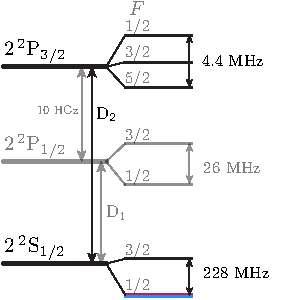
\includegraphics{fig-ai/li-levels-base.pdf}
    \hfill
    \addletter{140}{b}
    \includegraphics{fig-py/li6-zeeman.pdf}
    \hfill
    \addletter{140}{c}
    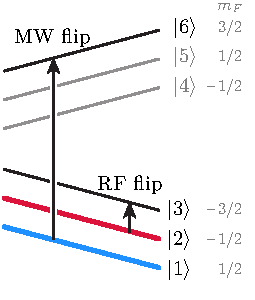
\includegraphics{fig-ai/li-levels.pdf}
    \caption{
        \textbf{${}^6$Li energy levels}. 
        a) Level diagram of the ground and 2P excited states of ${}^6$Li \cite{gehm_preparation_2003}. 
        b) Zeeman splitting of the hyperfine levels of the $2\, {}^2\mathrm{S}_{1/2}$ state in ${}^6$Li \cite{serwane_deterministic_2011, sibalic_arc_2017}. With dashed line was marked non-interacting regime for 1-2 mixture at 527 Gs. c) As different spin states for physics we consider state $\ket{1}$ and $\ket{2}$, but for imaging it is worth to flip them to close transitions.
        \red{Можно разделить (b), чтобы показать и расщепление для P32.}
    }
    \label{fig:li6levels}
\end{figure} % Optical scheme, atom preparation, probe configuration

\subsection{Image processing} \label{subsec:imaging-processing}
% !TEX root = ../master-thesis.tex


\begin{figure}
    \centering
    \addletter{125}{a}
    \includegraphics{fig-py/imaging-hist.pdf}
    \hfill
    \addletter{125}{b}
    \includegraphics{fig-py/imaging-base.pdf}
    \caption[Single-atom identification and image processing]{
        \textbf{Single-atom identification and image processing.}
        a) Histogram of peak intensities extracted from binarized and low-pass filtered images shows a bimodal distribution: the first peak corresponds to camera noise (black), the second corresponds to single atoms (red). The dashed line indicates the threshold used for atom identification.
        b) Image processing pipeline: Raw fluorescence image (left), binarization by intensity thresholding (center), and application of a low-pass filter (right) to reveal spatially localized atomic signals. 
        % \red{Для (a) можно добавить fit, показав что иногда случаются и два атома.}
    }
    \label{fig:imaging}
\end{figure}

% \textbf{Camera and detection regime.}  
The imaging system uses a Nüvü HNü512 EMCCD camera, chosen for its high sensitivity and low noise in the few-photon regime. At $\lambda = 671$~nm, the sensor achieves a quantum efficiency (QE) of approximately 94\%~\cite{kruip_design_2024}. The camera is operated in photon counting mode with EM gain up to 5000, enabling single-atom detection from just tens of detected photons. During a typical imaging sequence, each atom emits around 300 photons, of which approximately 30 are detected on the camera after collection and transmission losses.

% \textbf{Binarization and filtering pipeline.}  
To mitigate the excess noise factor (ENF) inherent in EM amplification and to suppress clock-induced charges (CICs), we apply a binarization scheme. A fixed threshold (typically $5\sigma_\text{read}$ above the baseline noise) is used to convert raw images into binary maps, where each pixel is marked as "bright" if it exceeds the threshold and "dark" otherwise. This removes ambiguity due to the stochastic gain distribution and allows images to be treated as photon arrival maps.  

To reduce high-frequency noise while preserving localized atomic signals, we apply a Gaussian low-pass filter with a tunable width (typically $\sigma = 7$ px, close to the diffusion scale). This smooths the binarized images and helps identify spatially coherent clusters corresponding to single atoms. 
% \red{Optionally, a denoising step based on a circular neighbor-count kernel can be applied after binarization; see Appendix for implementation details.}

% \textbf{Atom identification from local maxima.}  
We locate candidate atom positions by searching for local maxima in the filtered images. Since the imaging beam is symmetric and atoms are spatially separated (due to the tweezer geometry), each atom forms a compact signal peak. To distinguish real atoms from CIC-induced noise clusters, we construct a histogram of peak amplitudes and apply a classification threshold based on the bimodal structure (see Fig.~\ref{fig:imaging}). This provides a robust method for single-atom detection within each image.

% \textbf{Use of ROI and regular array geometry.}  
During this work, all experiments were performed with a regular tweezer array. This allows us to restrict image analysis to known regions of interest (ROIs) around each expected atom location. This prior knowledge significantly simplifies the classification problem: we identify the atom at a given site as present or absent based on the presence of a peak in the corresponding ROI. This enables more reliable classification than in fully general imaging tasks as in \cite{bergschneider_spin-resolved_2018}.

% \textbf{Implementation and contribution.}  
The entire image analysis pipeline (bias correction, binarization, optional denoising, filtering, and classification) was implemented by the author in Python. The resulting code is vectorized and supports batch processing of image sequences. While the core concepts draw from existing methods developed in~\cite{bergschneider_spin-resolved_2018}, the current implementation is adapted to the geometry and noise characteristics of our setup. 
% Notably, the simplification due to known array geometry enables efficient and accurate analysis suitable for high-throughput acquisition.
 % Thresholding, noise filtering, spatial resolution

\subsection{Spin-resolved detection} \label{subsec:imaging-spin}
% !TEX root = ../master-thesis.tex

\begin{figure}
    \centering
    \includegraphics{fig-py/imaging-spin-resolved.pdf}
    \caption{
        \textbf{Spin-resolved single-atom imaging.}
        Spatially separated $\sigma_+$ and $\sigma_-$ fluorescence is imaged onto two distinct regions of the camera. The binarization step identifies photon counts above a threshold, followed by a low-pass filter to extract spatially localized signals. Final spin states are assigned based on relative signal strength in each channel:
        \raisebox{-1pt}{\scalebox{1.5}{\textcolor{ublue}{\textbullet}}} -- $\ket{1}$, 
        \raisebox{-1pt}{\scalebox{1.5}{\textcolor{ured}{\textbullet}}} -- $\ket{2}$, 
        \raisebox{-1pt}{\scalebox{1.5}{\textcolor{uhole}{\textbullet}}} -- no atom.
    }
    \label{fig:spin-resolved}
\end{figure}


% \textbf{Single-shot spin resolution with spatial separation.}  
% Spin detection is implemented through a single-exposure fluorescence measurement, where the emitted light from atoms in $\ket{3}$ and $\ket{6}$ is directed to different regions of the camera. This spatial separation is achieved using a polarizing beam splitter (PBS) after the imaging objective, which splits $\sigma^+$ and $\sigma^-$ components. In our geometry, atoms in state $\ket{3}$ produce fluorescence in the upper-right region of the frame, while those in $\ket{6}$ appear in the lower-left (see Fig.~\ref{fig:spin-resolved}). The system is calibrated so that each site in the tweezer array corresponds to two fixed analysis regions—one per spin channel.

% \textbf{Filling detection.}  
% For each tweezer site, the signal is integrated within two predefined ROIs, each capturing the fluorescence from one spin channel. The presence and identity of an atom is determined by comparing the signals from the two channels. If the signal in only one ROI exceeds a detection threshold, the corresponding spin state ($\ket{3}$ or $\ket{6}$) is assigned. If neither region contains sufficient signal, the site is identified as empty. If both channels yield strong and spatially localized peaks, this is interpreted as the presence of two atoms in different spin states at the same site.

% \textbf{Fidelity estimation from single-atom preparation.}  
% To characterize the performance of spin-resolved detection, we use deterministic state preparation. In these experiments, each tweezer contains an atom with a known spin state ($\ket{3}$ or $\ket{6}$) with approximately 95\% probability, as determined independently via fluorescence-based atom counting~\cite{dux_optical_2023}, see Fig.~\ref{fig:spillingadd}. Additionally, some choosen ROIs are intentionally left empty to provide ground truth data for evaluating false positive rates.

% By applying the full detection pipeline to these experiments, we extract the rates of false positives (detecting an atom where none is present) and false negatives (failing to detect an atom where one exists). While the resulting classification accuracy depends on the overall filling fraction, the intrinsic detection characteristics (the false positive and false negative rates) are filling-independent. For a representative filling of 0.5, the resulting accuracy of spin-state assignment reaches 99\%. This performance level is sufficient for the current experiment stage.

% \textbf{Implementation and contribution.}  
% The complete processing pipeline for extracting spin-resolved occupancy data from camera images was implemented by the author. The classification algorithm builds on the same architecture used for unpolarized imaging but includes support for analyzing two spatially distinct fluorescence regions per site. The code is vectorized for efficient processing and can be extended to support additional spin channels or dynamic configurations.


\textbf{Single-shot spin resolution with spatial separation.} Spin detection is implemented through a single-exposure fluorescence measurement, where the emitted light from atoms in $\ket{3}$ and $\ket{6}$ is directed to different regions of the camera. This spatial separation is achieved using a polarizing beam splitter (PBS) after the imaging objective, which splits $\sigma^+$ and $\sigma^-$ components. In our geometry, atoms in state $\ket{3}$ produce fluorescence in the upper-right region of the frame, while those in $\ket{6}$ appear in the lower-left (see Fig.~\ref{fig:spin-resolved}). The system is calibrated so that each site in the tweezer array corresponds to two fixed analysis regions—one per spin channel.

\textbf{Filling detection.} For each tweezer site, the signal is integrated within two predefined ROIs, each capturing the fluorescence from one spin channel. The presence and identity of an atom is determined by comparing the signals from the two channels. If the signal in only one ROI exceeds a detection threshold, the corresponding spin state ($\ket{3}$ or $\ket{6}$) is assigned. If neither region contains sufficient signal, the site is identified as empty. If both channels yield strong and spatially localized peaks, this is interpreted as the presence of two atoms in different spin states at the same site.

\textbf{Fidelity estimation from single-atom preparation.} To characterize the performance of spin-resolved detection, we use deterministic state preparation. In these experiments, each tweezer contains an atom with a known spin state ($\ket{3}$ or $\ket{6}$) with approximately 95\% probability, as determined independently via fluorescence-based atom counting~\cite{dux_optical_2023}, see Fig.~\ref{fig:spillingadd}. Additionally, some chosen ROIs are intentionally left empty to provide ground truth data for evaluating false positive rates. By applying the vectorized processing pipeline (implemented by the author and building on the unpolarized imaging architecture) to these experiments, we extract the rates of false positives (detecting an atom where none is present) and false negatives (failing to detect an atom where one exists). The classification algorithm supports two spatially distinct fluorescence regions per site and can be extended to additional spin channels or dynamic configurations. While the resulting classification accuracy depends on the overall filling fraction, the intrinsic detection characteristics (the false positive and false negative rates) are filling-independent. For a representative filling of 0.5, the resulting accuracy of spin-state assignment reaches 99\%. This performance level is sufficient for the current experiment stage. % Two-step imaging, state identification, fidelity

\subsection{Spin manipulation} \label{subsec:imaging-flip}
% !TEX root = ../master-thesis.tex

\textbf{Introduction and motivation.}
Manipulating the internal spin state of ultracold atoms is an essential element in quantum simulation experiments, particularly for us in context of deterministic state preparation and spin-resolved imaging.
Two widely employed methods for achieving controlled spin transitions in ultracold atomic systems are the Landau-Zener transition and coherent resonant $\pi$-pulse. The Landau-Zener approach involves adiabatically sweeping either the frequency of a driving field or the magnitude of a magnetic field across a spin-resonance. It has been widely applied due to its inherent robustness against small deviations in experimental parameters such as magnetic field fluctuations and frequency drifts. In contrast, the $\pi$-pulse method achieves spin flips by applying a resonant electromagnetic field pulse of precise duration, determined by the corresponding Rabi frequency. Although $\pi$-pulses offer considerably faster spin-flip operations, their fidelity is strongly sensitive to precise calibration of pulse duration, intensity, and frequency detuning, making them more susceptible to experimental noise and parameter instabilities.

Within the context of the current experiment, spin manipulation techniques serve two primary functions. Firstly, flipping atomic spins to stretched states enhances the efficiency of spin-resolved fluorescence imaging. Secondly, selective spin flips are integral to preparation protocols such as spin-selective spilling, allowing controlled removal of atoms in specific spin states. While the Landau-Zener method provided a practical starting point during initial setup stages (mainly due to its robustness against parameter variations) the progression toward faster experimental cycles motivated a transition towards using resonant $\pi$-pulses.

In the following paragraphs, the theoretical foundations of both Landau-Zener and $\pi$-pulse spin manipulation methods are described in detail. A comparative analysis then outlines their respective advantages and limitations in the presence of parameter noise, ultimately justifying the preferred choice adopted in this work.


\textbf{Landau-Zener transition.}
The Landau-Zener transition \cite{landau_zur_1932,zener_non-adiabatic_1997} describes the non-adiabatic transition between two quantum states when the energy separation between these states is varied linearly in time. The Hamiltonian governing the dynamics of a two-level system undergoing such a process can be expressed as:
\begin{equation}
H_{\text{LZ}}(t) = \frac{\hbar}{2}
\begin{pmatrix}
\Delta(t) & \Omega \\
\Omega & -\Delta(t)
\end{pmatrix},
\label{eq:LZ_Hamiltonian}
\end{equation}
where $\Delta(t)$ represents the instantaneous detuning between the system resonance and the external driving field, and $\Omega$ denotes the coupling strength (Rabi frequency) between the two states. Typically, the detuning is varied linearly as $\Delta(t) = \alpha t$, with $\alpha$ defined as the rate of change of detuning.

The transition probability $P_{\text{LZ}}$ between the two states, derived analytically under the assumption of a linear sweep and constant coupling, is given by the well-known Landau-Zener formula:
\begin{equation}
P_{\text{LZ}} = 1 - \exp\left(-\frac{\pi \Omega^2}{2\alpha}\right).
\label{eq:LZ_probability}
\end{equation}
From Eq.~\eqref{eq:LZ_probability}, it follows that the transition probability depends explicitly on the ratio of the coupling strength squared, $\Omega^2$, to the rate of detuning change, $\alpha$. For slow sweeps ($\alpha \ll \Omega^2$), the system undergoes nearly complete transitions ($P_{\text{LZ}}\rightarrow1$), whereas faster sweeps result in incomplete transitions and correspondingly reduced fidelity.

An important experimental advantage of the Landau-Zener method lies in its robustness against fluctuations in experimental parameters, such as variations in the magnitude of the magnetic field or the exact driving frequency. If the magnetic field is swept across a hyperfine transition, slight deviations in the magnetic field gradient or frequency tuning rate will only minimally affect the transition fidelity due to the exponential nature of Eq.~\eqref{eq:LZ_probability}. Such robustness proves particularly valuable in experimental settings, where shot-to-shot variations in magnetic field magnitude or small frequency drifts inevitably occur.

% Furthermore, Landau-Zener transitions can be implemented either by sweeping the frequency of an applied microwave or radiofrequency field across the resonance or equivalently by sweeping the magnetic field, which shifts the resonant frequency via the Zeeman effect. Both approaches yield equivalent results, and the choice between them is typically dictated by experimental convenience and technical considerations related to equipment availability and stability.

Despite the robustness of Landau-Zener transitions, a notable drawback is the relatively long timescale ($\sub{t}{LZ} \gg 1/\Omega$) required to achieve high transition.  In the subsequent section, a detailed discussion of the alternative approach, resonant $\pi$-pulse spin manipulation, will be presented, highlighting contrasting properties and the sensitivity of each technique to experimental noise sources.


\textbf{Rabi $\pi$-pulse.}
An alternative approach for inducing spin-state transitions in ultracold atomic systems is the resonant Rabi oscillation method, commonly referred to as the $\pi$-pulse technique. This method exploits coherent resonant driving of the transition between two spin states, enabling deterministic and rapid population transfer.

The dynamics of a two-level quantum system under resonant excitation is described by the same Hamiltonian \eqref{eq:LZ_Hamiltonian} with implied $\Delta = \const$. Specifically, applying the driving field for the duration $t_\pi = \pi/\Omega$ with $\Delta=0$, the system undergoes a complete inversion of the spin populations, realizing a perfect spin-flip operation from state $\ket{1}$ to state $\ket{2}$, or vice versa. Main advantage is that $t_\pi \ll \sub{t}{LZ}$, main limitation is that deviations from the exact resonance condition ($\delta \neq 0$), or inaccuracies in pulse duration and field amplitude, reduce the transition fidelity. The fidelity of the spin flip under a non-zero detuning is analytically described by the generalized Rabi oscillation formula:
\begin{equation}
P_{\pi} = \frac{\Omega^2}{\Omega^2+\delta^2}\sin^2\left(\frac{\sqrt{\Omega^2+\delta^2}}{2}t_{\pi}\right).
\label{eq:pi_fidelity}
\end{equation}
Shot-to-shot fluctuations, particularly in magnetic fields, directly introduce variations in resonance conditions, which result in systematic and random errors in the spin-flip fidelity. 
% Consequently, achieving consistently high fidelity with $\pi$-pulses demands stringent experimental stabilization and calibration protocols.


% In summary, the $\pi$-pulse technique enables fast, deterministic spin flips but requires high precision and stable experimental conditions. The interplay between speed, fidelity, and sensitivity to noise thus determines the appropriateness of this technique for specific experimental goals, as will be further analyzed in the subsequent comparative section.

\subsection{Conclusion} \label{subsec:imaging-conclusion}
% !TEX root = ../master-thesis.tex

This chapter has detailed the implementation of a spin-resolved free-space imaging system for ${}^6$Li atoms in an optical tweezer array. The approach is tailored to fast-cycle experiments and leverages the intrinsic spacing of the array to bypass the need for sub-micron spatial resolution.

The free-space fluorescence method was motivated both conceptually and practically, with an emphasis on momentum-space dynamics during imaging. Theoretical considerations based on the SSH model support the use of alternating beam sequences to reduce spatial diffusion, thereby improving localization fidelity.

The optical setup includes two independent laser beams driving stretched-state cycling transitions, with modulation handled via AOMs and synchronized control electronics. A distribution board was constructed to combine and route the beams, ensuring symmetric delivery to the atoms.

The image analysis pipeline applies binarization and spatial filtering to extract single-atom signals from low-flux data. The use of fixed array geometry enables simplified region-of-interest (ROI) analysis and improves classification reliability. All components of the processing chain are implemented in a parallelized, vectorized framework to support high-throughput acquisition.

Spin information is extracted by mapping fluorescence from $\sigma^+$ and $\sigma^-$ transitions to distinct regions on the camera. A per-site classification algorithm assigns spin states based on signal strengths in these regions. Validation against calibrated single-atom counted experiments yields a classification accuracy of approximately 99\% under typical experimental conditions.

These techniques constitute a fast and reliable imaging solution suitable for experiments requiring spin-resolved readout, and are readily extensible to future array sizes and imaging geometries.



\newpage
% --------------------------------------------------------------------------------------
\section{Tweezer array system} \label{sec:tweezer}
% --------------------------------------------------------------------------------------

\subsection{Introduction} \label{subsec:state-prepation-overview}
% !TEX root = ../master-thesis.tex


Quantum simulation with ultracold atoms requires precise control over initial many-body states to access regimes beyond thermal equilibrium and study specific quantum phenomena. Traditional loading methods from magneto-optical traps or degenerate gases produce stochastic particle distributions that limit the ability to prepare designer initial states necessary for studying complex quantum phases, far-from-equilibrium dynamics, or engineered many-body Hamiltonians. The development of deterministic loading and manipulation techniques has become essential for advancing quantum simulation capabilities, particularly in fermionic systems where spin degrees of freedom play crucial roles.

\textbf{Traditional Loading Methods and Limitations.} 
Conventional approaches to loading optical lattices rely on transferring atoms from magneto-optical traps (MOTs) or pre-cooled atomic clouds into the periodic potential created by interfering laser beams. In these methods, atoms are first captured and cooled in a MOT, then typically transferred to a magnetic or optical dipole trap for further evaporative cooling to quantum degeneracy. The resulting degenerate gas is subsequently loaded into the optical lattice by adiabatically ramping up the lattice depth while the harmonic confinement is maintained or modified.

This standard loading procedure suffers from fundamental limitations arising from its stochastic nature. When atoms are loaded from a thermal or quantum degenerate cloud, the number of particles at each lattice site follows Poissonian statistics, determined by the local chemical potential and temperature. For a uniform system at chemical potential $\mu$, the average site occupation is given by the local density, but fluctuations are unavoidable. Experimental demonstrations of Mott insulators in various atomic species have confirmed these statistical limitations. Early experiments with $^{87}$Rb achieved Mott insulator phases with site occupancy fidelities limited to approximately \red{60-70\%} for unit filling, primarily due to thermal fluctuations and imperfect adiabatic loading. Similar limitations were observed in fermionic $^{40}$K and $^6$Li systems, where achieving high-fidelity band insulators required very low temperatures and careful control of interaction strengths through Feshbach resonances.
% In the Mott insulator regime at unit filling, where on average one atom occupies each site, the probability of finding exactly $n$ atoms at a given site follows $P(n) = e^{-\langle n \rangle}\langle n \rangle^n/n!$ where $\langle n \rangle \approx 1$.
% This results in approximately 37\% empty sites, 37\% singly occupied sites, 18\% doubly occupied sites, and 8\% higher occupancies even under optimal conditions.


The harmonic confinement typically present in these experiments further complicates state preparation by creating spatial inhomogeneity. The varying local chemical potential across the trap leads to the formation of concentric "wedding cake" structures with different filling factors in different regions, making it difficult to achieve uniform occupancy over extended areas. While techniques such as digital micromirror device (DMD) compensation can flatten the trapping potential, the fundamental Poissonian loading statistics remain unchanged.

For spin-selective loading, traditional methods face additional challenges. Starting from a thermal cloud or degenerate gas, both spin components are typically loaded simultaneously with correlated fluctuations. Achieving specific spin patterns or controlled spin imbalances requires post-loading manipulation through techniques such as selective removal or magnetic field gradients, which can introduce heating and reduce overall atom numbers.

These limitations have motivated the development of alternative approaches that can circumvent the statistical nature of traditional loading and provide deterministic control over both spatial and spin degrees of freedom in lattice systems.


\textbf{SLM and DMD for Site-Selective Manipulation.}
The limitations of stochastic loading motivated the development of post-loading manipulation techniques using spatial light modulators (SLMs) and digital micromirror devices (DMDs) to achieve precise control over atomic distributions in optical lattices. These approaches enable site-selective addressing and manipulation after initial loading, allowing experimenters to "sculpt" desired atomic configurations from the initial Poissonian distribution.

Digital micromirror devices offer fast switching times and straightforward implementation for creating programmable optical potentials. DMDs consist of arrays of individually controllable micro-mirrors that can be rapidly reconfigured to create binary intensity patterns, with grayscale levels achieved through temporal modulation or spatial dithering techniques. The Greiner group pioneered the use of DMDs for quantum gas microscopy, demonstrating the ability to project arbitrary potential landscapes onto Mott insulators with microsecond reconfiguration times~\cite{mazurenko_cold-atom_2017}. Their approach enabled dynamic manipulation of lattice geometries and compensation of harmonic confinement to create uniform "box" potentials with improved loading uniformity.

A particularly powerful technique is the "microwave knife" method for site-selective atom removal. This approach combines magnetic field gradients with spatially selective microwave addressing to remove atoms from specific lattice sites with high precision. The technique exploits position-dependent energy shifts for atomic hyperfine states created by magnetic gradients, making each lattice site resonant with a slightly different microwave frequency. Weitenberg et al. first demonstrated this method in $^{87}$Rb quantum gas microscopes, achieving single-site addressing fidelity of approximately 95\%~\cite{weitenberg_single-spin_2011}. The procedure involves applying a magnetic field gradient across the lattice, then using a focused microwave beam to selectively drive transitions at chosen sites, transferring atoms to states that can be subsequently removed using resonant light.

Extensions of the microwave knife technique have enabled the creation of arbitrary patterns of holes in Mott insulators and the realization of custom lattice geometries. Achieved fidelities for pattern creation typically range from 85-95\%, limited primarily by imperfect selectivity of the microwave addressing and residual heating. DMD-based approaches have enabled rapid pattern switching and dynamic manipulation during experiments, with reconfiguration times on microsecond timescales enabling studies of quantum quenches and thermalization dynamics~\cite{choi_exploring_2016}.

% However, these site-selective manipulation techniques share a fundamental limitation: they are primarily "subtractive" methods that can remove atoms from occupied sites but cannot add atoms to empty sites. While they enable precise sculpting of atomic patterns from an initial filled state, achieving arbitrary configurations requires starting with sufficient occupancy everywhere in the pattern. This constraint limits the types of initial states that can be prepared and often requires sacrificing atoms to achieve the desired configuration, reducing the overall system size. Additionally, the fidelity is fundamentally limited by the initial Poissonian loading statistics, as sites that are initially empty cannot be filled using these methods.

% Despite these limitations, SLM and DMD-based manipulation techniques represented a crucial advancement in experimental control over many-body quantum systems, establishing the groundwork for more sophisticated state preparation techniques and demonstrating the importance of precise initial state control for quantum simulation applications.


\textbf{Spin-Selective State Preparation.} Control over the internal spin degrees of freedom of atoms in optical lattices is essential for quantum simulation of magnetic systems and strongly correlated electron models. For $^6$Li, the two lowest hyperfine ground states $|F=\frac{1}{2}, m_F=\pm\frac{1}{2}\rangle$ (commonly denoted $|\uparrow\rangle$ and $|\downarrow\rangle$) provide a natural spin-1/2 system.

Global optical pumping represents the most fundamental approach, transferring populations to a desired hyperfine state with fidelities exceeding 99\%. However, this technique lacks spatial selectivity, preparing uniform spin states across the entire sample. Radiofrequency and microwave transitions enable coherent manipulation of spin states after loading, with spatial selectivity achieved by combining RF pulses with magnetic field gradients~\cite{weitenberg_single-spin_2011}. This approach uses position-dependent Zeeman shifts to make each lattice site resonant with different RF frequencies, enabling single-site spin flips with approximately 95\% fidelity.

Spin-selective optical potentials provide another route by creating different AC Stark shifts for the two spin states, allowing spatial separation or selective manipulation of spin components. The widely adopted "blast" technique exploits distinct optical transitions of different hyperfine states to selectively remove atoms of one spin while leaving the other unaffected. For $^6$Li in magnetic fields, resonant light tuned to one transition ejects atoms in that state while the other remains trapped due to large detuning. Achieved fidelities for selective removal typically exceed 98\%.

Site-resolved spin preparation combining magnetic field gradients with focused optical beams enables preparation of complex spin patterns with single-site resolution. Demonstrations include preparation of antiferromagnetic order in 2D Fermi-Hubbard systems~\cite{mazurenko_cold-atom_2017} and controlled doublon dynamics~\cite{covey_doublon_2016}, achieving stable pair states with high precision.

However, these lattice-based techniques face fundamental limitations compared to constructive approaches. They operate on pre-existing atomic distributions, limiting achievable configurations to modifications of initial Poissonian loading. Empty sites cannot be filled selectively, and achieving specific atom number and spin combinations requires statistical averaging. Additionally, many methods involve heating mechanisms that reduce system coherence, and spin-selective removal necessarily reduces total atom number.

Despite these limitations, lattice-based spin preparation techniques enabled the first demonstrations of engineered magnetic states in ultracold atom systems and established foundations for understanding many-body spin dynamics in optical lattices.


\textbf{Tweezer-Based Loading.} Optical tweezers represent a paradigm shift from stochastic to deterministic loading methods, enabling precise "bottom-up" assembly of many-body quantum systems with arbitrary initial configurations. Unlike traditional loading approaches that rely on statistical distributions, tweezer-based methods provide constructive control over both spatial and internal degrees of freedom, circumventing the fundamental limitations of Poissonian statistics.

The core principle involves using tightly focused laser beams to create microscopic dipole traps that can capture and manipulate individual atoms. The first deterministic preparation of few-fermion systems using optical tweezers with $^6$Li achieved ground-state preparation of 1 to 10 particles with fidelities of approximately 90\%~\cite{serwane_deterministic_2011}. The technique relies on careful control of trap depth and interactions, combined with a "spilling" method that enables exact atom number selection.

The spilling technique exploits the quantized energy levels of fermions in the tight confinement of optical tweezers. By adiabatically reducing the trap depth, atoms occupying the highest energy levels become unbound and escape, while those in lower levels remain trapped. Due to Pauli exclusion, each quantum level accommodates at most one atom per spin state, allowing precise control over the final atom number by selecting the appropriate trap depth. Single-atom loading fidelities exceeding 99\% have been demonstrated in individual tweezers for various atomic systems.

A particularly powerful extension for $^6$Li involves spin-selective spilling using magnetic field gradients. At specific magnetic field strengths, the two hyperfine ground states $|\uparrow\rangle$ and $|\downarrow\rangle$ exhibit different magnetic moments, causing only one spin state to experience significant forces from applied magnetic gradients. This differential response enables selective removal of one spin component while leaving the other unaffected. By carefully tuning the magnetic field and applying controlled gradients during spilling, experimenters can deterministically prepare tweezers containing specific configurations: empty sites, single $|\uparrow\rangle$ atoms, single $|\downarrow\rangle$ atoms, or spin-paired doublons.

The constructive nature of tweezer-based loading provides decisive advantages over subtractive lattice manipulation techniques. Arbitrary spatial patterns can be assembled without requiring initial occupancy at every target site, and specific atom numbers can be placed at chosen locations regardless of initial distribution. This enables preparation of complex initial states that would be statistically unlikely through thermal loading, such as perfect antiferromagnetic order or exotic spin patterns.

Scalability has improved dramatically through advances in optical control systems. Modern implementations using spatial light modulators and digital micromirror devices can generate and control hundreds to thousands of individual tweezers simultaneously~\cite{stuart_single-atom_2018}. Recent demonstrations have shown continuous operation of large-scale atom arrays with more than 1000 atoms~\cite{gyger_continuous_2024}, indicating potential for scaling to system sizes relevant for quantum simulation applications.

The combination of deterministic number control with spin selectivity enables preparation of initial states crucial for studying strongly correlated quantum systems. Controlled few-fermion preparation has been used to realize antiferromagnetic Heisenberg spin chains~\cite{murmann_antiferromagnetic_2015}, demonstrating how precise initial state control enables access to specific many-body quantum phases. The ability to prepare exact Fock states with predetermined spin configurations opens possibilities for studying quantum phase transitions and exotic quantum phases requiring specific initial conditions.

The integration of tweezer arrays with optical lattices represents a powerful hybrid approach. Atoms can be initially assembled in a defect-free tweezer array with the desired spatial and spin configuration, then adiabatically transferred into an optical lattice for many-body dynamics studies. This combination preserves deterministic initial state preparation while providing the periodic potential structure necessary for implementing specific model Hamiltonians. Advanced control capabilities demonstrated in Rydberg tweezer arrays~\cite{bornet_enhancing_2024} show the potential for even more sophisticated manipulation protocols applicable to fermionic systems.

The advantages of tweezer-based loading extend beyond simple state preparation to enable entirely new classes of quantum simulation experiments. The ability to prepare systems with exact atom numbers and spin configurations removes statistical uncertainties that have limited previous studies, enabling precise benchmarking of theoretical predictions and access to quantum phases that require specific particle numbers or spin arrangements.

\subsection{Acousto-optic deflector} \label{subsec:aodconcept}
% !TEX root = ../master-thesis.tex

\begin{figure}
    \centering
    % 
    \addletter{140}{a} 
    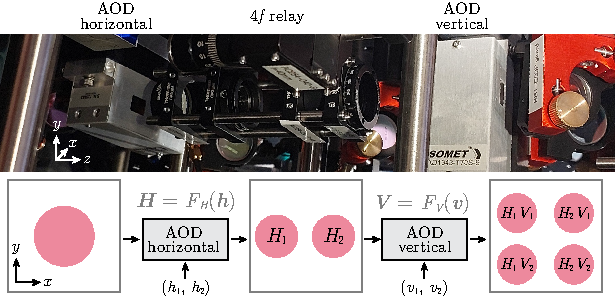
\includegraphics{fig-ai/crossed-aod.pdf}
    \hfill
    \addletter{140}{b} 
    \includegraphics{fig-py/crosstalk-camera.pdf}
    % 
    \newline
    \phantom{42}
    \newline
    % 
    \addletter{115}{c}
    \raisebox{1cm}{\includegraphics{fig-py/crosstalk-camera-img.pdf}}
    \phantom{42}
    \addletter{115}{d}
    \includegraphics{fig-py/crosstalk-camera-amp.pdf}  
    \phantom{42}
    \addletter{115}{e}
    \includegraphics{fig-py/crosstalk-camera-res.pdf}
    % 
    \caption{
        \textbf{Tweezer array control using orthogonal AODs.}
        (a) Experimental setup: two orthogonal AODs generate a 2D tweezer array. The applied harmonic amplitudes $h_i$, $v_j$ define the output intensities $H_i = F_H(h)$ and $V_j = F_V(v)$ in horizontal and vertical directions, respectively. 
        (b) Crosstalk matrix $F'$ reconstructed via linear regression from camera images, showing how modulation of one harmonic affects others. 
        (c) Example of measured intensity distribution at uniform input amplitudes ($h_i = v_j = 0.9$), illustrating imbalance in the resulting pattern. 
        (d) The total intensity $\Lambda = \sum_{ij} H_i V_j$ scales linearly with the mean input amplitude. 
        (e) Residuals of the linear model (fitted in the range $[0.85, 0.95]$) are normally distributed. 
        All data were obtained in this work using direct camera-based measurements.
    }
    \label{fig:control}
\end{figure}


Optical tweezer arrays provide a flexible platform for preparing ultracold atomic systems with site-resolved control. By trapping individual atoms in focused laser beams, it becomes possible to initialize many-body states with controlled geometry, low entropy, and tunable local parameters.

In our setup, a two-dimensional array of tweezers is created using two orthogonal acousto-optic deflectors (AODs). Each AOD diffracts multiple beams along one axis, and their intersection forms the full array. The resulting intensity at site $(i,j)$ factorizes as $P_{ij} = H_i V_j$, where $H_i$ and $V_j$ are set by the drive amplitudes applied to each AOD. This structure simplifies calibration and allows fast control of the entire array using a small number of parameters.

Compared to holographic or lattice-based approaches, the AOD system offers rapid reconfigurability and independent control of individual traps. This enables preparation of custom spin and density patterns, as well as dynamic manipulation during the experimental sequence. Such capabilities are useful, for example, for initializing specific configurations, removing defects, or performing spatially selective operations before loading atoms into an optical lattice for further evolution.

\textbf{AOD operation.} Each AOD consists of a crystal driven by a piezoelectric transducer. An incoming laser beam $(\vc{k}_{\mathrm{in}}, \omega_{\mathrm{in}})$ interacts with the induced acoustic wave $(\vc{q}, \Omega)$ via Bragg diffraction, producing an outgoing beam $(\vc{k}_{\mathrm{out}}, \omega_{\mathrm{out}})$:
\begin{equation*}
    \vc{k}_{\mathrm{out}} = \vc{k}_{\mathrm{in}} + \vc{q}, \qquad \omega_{\mathrm{out}} = \omega_{\mathrm{in}} + \Omega.
\end{equation*}
The frequency $\Omega$ determines the deflection angle $\theta$ through the Bragg condition, while the amplitude of the RF signal controls the diffracted optical power. Each RF tone can be described by a triple $(\Omega_j, a_j, \varphi_j)$, corresponding to its frequency, amplitude, and phase. Applying a set of such tones to an AOD results in a superposition of multiple diffracted beams, with the amplitude $a_j$ determining the power in each beam and the phase $\varphi_j$ influencing their relative coherence.


\textbf{Factorized intensity distribution.} 
To create 2D arrays, we combine two AODs oriented along orthogonal axes (fig.~\ref{fig:control}a), as described in~\cite{culemann_construction_2024}.
Each axis is driven by a set of RF tones. In the paraxial approximation, the resulting 2D intensity pattern can be written as a rank-1 product of two vectors:
\begin{equation*}
    P_{ij} = H_i V_j,
\end{equation*}
where $H_i$ and $V_j$ correspond to the powers of individual beams generated by the horizontal and vertical AOD, respectively. The factorization of the output power can be verified via:
\begin{equation}
\label{eq:factorisability}
    P \overset{\mathrm{SVD}}{=} \textstyle \sum_r \Lambda_r \vc{H}_r \vc{V}_r\T,
    \hspace{10 mm} 
    \text{factorisability} = \Lambda_0 / \sum_r \Lambda_r 
\end{equation}
which provides a natural measure of factorization. For arrays ranging from $2\times2$ to $10\times10$, the factorisability measure $\Lambda_0 / \sum_r \Lambda_r$ is consistently above $0.99$. For the $4\times4$ array used in most of our experiments, we obtain a typical value of $0.997(1)$.

\textbf{Tweezer array control.} The tweezer output beam powers are nonlinear functions of the input amplitudes $\vc{a}$:
\begin{equation}
    \label{eq:taylerexp}
    P_j = F_j(\vc{a}) = \cancel{F_j(\vc{0})} + F'_{ji} a_i + \tfrac{1}{2} F''_{j i_1 i_2} a_{i_1} a_{i_2} + \ldots
\end{equation}
The goal is to control\footnote{
    For amplitudes in the range $a_i \in [0.7, 1.0]$, we find that a linear or quadratic approximation suffices. In practice, we reconstruct the Jacobian matrix $F'_{ji}$ using camera-based calibration, as discussed in Sec.~\ref{subsec:control}.
} the full matrix $P_{ij}$ using only two sets of parameters: horizontal amplitudes $\vc{h}$ and vertical amplitudes $\vc{v}$. 

It will later be necessary to reconstruct $(H_i, V_j)$ from measured intensity distribution $P_{ij}$, so it is convenient to choose a factorized model $P_{ij} = \Lambda H_i V_j$, with the normalization:
\begin{equation*}
    \sum_i H_i = \sum_j V_j = 1, \hspace{5 mm} \sum_{ij} P_{ij} = \Lambda.
\end{equation*}
This allows for an explicit decomposition:
\begin{equation}
    \textstyle
    \frac{1}{\Lambda} \sum_j P_{ij} = H_i \sum_j V_j = H_i,
    \hspace{5 mm} 
    \frac{1}{\Lambda} \sum_i P_{ij} = V_j \sum_i H_i = V_j,
    \hspace{5 mm} 
    \sum_{ij} P_{ij} = \Lambda,
    \label{uv-decomposition}
\end{equation}
which is fully equivalent to a rank-1 SVD of $P_{ij}$.

It is worth noting that, as shown in Fig.~\ref{fig:control}d, the total scale parameter $\Lambda$ defined in this way is proportional to the total input amplitude, $\sub{a}{sum} = \sum_j h_j + \sum_j v_j$. This effectively decouples local balancing from global power constraints, simplifying the control problem.

% \grey{This allows us to adjust the global scale $\Lambda$ (via a shared AOM or pre-AOD attenuation) and balance individual amplitudes using only two $n$-dimensional vectors.}
 % Tweezer arrays as control tool, overview

\subsection{Optical setup}
% !TEX root = ../master-thesis.tex

\begin{figure}
    \centering
    \includegraphics{fig-ai/preparation-seq.pdf}
    \caption{
        \textbf{Experimental sequence for deterministic atom number preparation.} 
        After loading a spin-balanced mixture into a crossed ODT from the MOT, we perform two-stage evaporation in the ODT. The atoms are then transferred into an optical tweezer via an adiabatic ramp. Further evaporation is carried out in the tweezer before executing the spilling procedure. Spilling takes place at 527\,G and a magnetic field gradient of 20\,G/cm to remove atoms above the spill level. The full sequence enables high-fidelity few-body preparation within a sub-2\,s cycle time. A detailed description can be found in~\cite{culemann_construction_2024}.
    }
    \label{fig:preparationseq}
\end{figure}


% \textbf{Acousto Optic Deflector (AOD)}. AOD, как и AOM, состоит из кристалла, который модулируется пьезоэлементом. Проходящие через кристалл фотоны $(\sub{\vc{k}}{in}, \sub{\omega}{in})$ рассеиваются на фононах $(\vc{q}, \Omega)$ via Bragg diffraction. To have higher efficiency we need to satisfy Bragg condition (проверить и добавить источник)
% \begin{equation*}
% 	\sub{n}{sc} q = \sub{k}{in} \sin(\theta),
% \end{equation*}
% \grey{где $\theta$ это угол между $\vc{k}$ и нормалью к $\vc{q}$} \red{(добавить рисунок)}. Внутри AOD находится несколько пьезоэлементов, к которым ведут провода подобранной длины так, чтобы при изменение частоты $\Omega$ направление $\vc{q}$ менялось соответсвующим Bragg condition образом. Это помогает улучшить диффракционную эффективность \grey{(добавить определение или ссылку)} AOD. На выходе полуются $(\sub{\vc{k}}{out}, \sub{\omega}{out}) = (\sub{\vc{k}}{in}+\vc{q}, \sub{\omega}{in} + \Omega)$. 
% Имея набор частот в модулирующем сигнале $(\vc{q}_j, \Omega_j)$ получим на выходе набор лучей
% \begin{equation*}
% 	(p_j, \vc{k}_j, \omega_j) = (F_j(\vc{a}, \sub{\vc{\omega}}{in}), \sub{\vc{k}}{in}+\vc{q}_j, \sub{\omega}{in} + \Omega_j),
% \end{equation*}
% c мощностью в каждом луче на выходе $p_j$. Регулируя вектор амплитуд $\vc{a}$, подающихся в AOD можно контролировать выходную мощность $\vc{p}$. 



\textbf{Beam collimation and polarization.} The tweezer array is formed by delivering light from a fiber outcoupler and collimating it with an $f = 40\,\mathrm{mm}$ achromatic lens mounted on a translation stage for precise control. To ensure efficient diffraction through the acousto-optic deflectors (AODs), horizontal polarization is set using a $\lambda/2$ waveplate and a polarizing beam splitter (PBS). Correct alignment of the PBS is verified by tracking the beam position on a camera before and after insertion.

\textbf{Acousto-optic deflectors and relay imaging.} The array is generated using a pair of orthogonally mounted AODs, each mounted on custom blocks to maintain a common beam height of 100\,mm. The beam is guided into the first AOD using two mirrors, and its alignment is optimized to maximize both transmission and diffraction efficiency (typically exceeding 90\% at 65\,MHz). The two AODs are connected via a 4f relay built from achromatic lenses in a 30\,mm cage system. Precise positioning is achieved by aligning the relay externally using collimated light and checking for minimal wavefront distortion on a shear plate. An iris at the Fourier plane of the relay filters out the zeroth diffraction order.

\textbf{Telescope and beam expansion.} After the second AOD, the beam is expanded using a telescope consisting of $f = 150\,\mathrm{mm}$ and $f = 500\,\mathrm{mm}$ lenses. The alignment ensures that the beam is collimated and centered on both lenses. The position of the second lens is mechanically fixed, while the telescope length is adjusted via mirror positions to achieve good collimation, verified with a shear plate. The zeroth-order beam after the second AOD is blocked at the intermediate focus.

\textbf{Monitoring and power balancing.} A flip mirror is installed in the beam path to optionally redirect the light into a monitoring camera without disturbing the main optical alignment. This enables fast access to the tweezer array profile during alignment or balancing procedures.

We avoid using a back-side polished mirror for beam sampling in front of the camera. Although commonly employed for its simplicity, such mirrors introduce (\red{? add measured data: october 2024}) spatially varying interference fringes due to reflections from different internal surfaces of the substrate. These fringes distort the measured intensity distribution, especially for rays entering the camera at different angles and positions. This effect becomes critical when calibrating the response of the AODs, as it leads to systematic errors in measured beam uniformity. Instead, we sample the beam with a removable flip mirror that fully redirects the beam, ensuring an undistorted and angle-independent intensity profile at the camera plane.
 % AODs, array generation, optical layout

\subsection{State preparation} \label{subsec:state-prepation}
% !TEX root = ../master-thesis.tex


% \textbf{Tweezer loading.} 
We begin by preparing a spin-balanced mixture in the two lowest hyperfine states, $|1\rangle$ and $|2\rangle$, using a compressed magneto-optical trap (MOT). The atoms are initially loaded into a crossed ODT, where we perform evaporative cooling. This follows closely the sequence described in~\cite{culemann_construction_2024}.

After cooling, the atoms are transferred into a tightly focused optical tweezer potential. The loading process relies on the so-called \emph{dimple trick}~\cite{zurn_few-fermion_2012}, where a tightly confined but deep tweezer potential is superimposed onto the wider ODT reservoir. Because the tweezer affects only a small region of the total cloud, the global temperature $T$ remains approximately unchanged, while the local chemical potential is enhanced. In this regime, the average occupation number $\bar{n}(E_i)$ of a single-particle state $i$ with energy $E_i$ follows the Fermi-Dirac distribution:
\begin{equation}
    \bar{n}(E_i) = \frac{1}{e^{(E_i - \mu)/k_B T} + 1}.
\end{equation}
If the energy gap between the ground state $E_0$ and the Fermi energy $E_F$ is increased such that $(E_0 - E_F) / k_B \gg T$, then $\bar{n}(E_0) \rightarrow 1$. This ensures near-unity occupation of the lowest level, which provides an ideal starting point for deterministic preparation. In our experiment, this condition is achieved by ramping on the tweezer adiabatically while continuing evaporation inside the tweezer. The full loading and cooling sequence is depicted in Fig.~\ref{fig:preparationseq}.

% \textbf{Deterministic few-body preparation via spilling.} 
To isolate a well-defined number of atoms in the lowest motional states of the tweezer, we use the \emph{spilling technique}, as described in~\cite{zurn_few-fermion_2012, holten_pauli_2022}. This method relies on tilting the potential with a magnetic field gradient and reducing the trap depth to allow atoms above a threshold energy to tunnel out. 
The resulting states are shown in Fig.~\ref{fig:preparation}.
% The energy levels and wavefunctions of the effective 1D potential under combined optical and magnetic fields were obtained numerically using a finite-difference method and the Thomas algorithm.

The spilling sequence is performed at a magnetic field of 527\,G, where the two spin states are nearly non-interacting. A magnetic field gradient of 20\,G/cm creates a linear tilt, and the tweezer power is lowered to a value that sets the spill threshold. After a short tunneling time, the trap depth is ramped back up to recapture the remaining atoms. By empirically optimizing these parameters, we achieve deterministic preparation of two atoms per tweezer with a fidelity of 90\,\%. This sequence results in high-fidelity preparation within a total experimental cycle time of less than 2\,s.



\begin{figure}
    \centering
    \includegraphics{fig-py/step-plot-2d.pdf}
    \caption[2D step plot]{
        \textbf{2D step plot.}
        Measured 2D step plot as a function of tweezer power and magnetic field gradient. Each point indicates the average atom number obtained for a given combination of parameters. This map confirms that for any spill power, a suitable magnetic gradient can be found to achieve a desired quantized atom number.
    }
    \label{fig:spillingadd-2d}
\end{figure}

 % Loading, cooling, spilling in single tweezer

\subsection{Tweezer control} \label{subsec:control}
% !TEX root = ../master-thesis.tex

\textbf{Frequency to position mapping.}
To extract the local intensities $P_{ij}$ from camera images, we need to determine which pixels correspond to which tweezer sites. For this purpose, we define an affine transformation from the drive frequency space $(\omega_{\mathrm{hor}}, \omega_{\mathrm{ver}})$ to image plane coordinates $(x, y)$:
\begin{equation*}
    \vc{r} = H \vc{\omega},
    \hspace{5 mm} \Leftrightarrow \hspace{5 mm} 
    \begin{pmatrix}
        x \\ y
    \end{pmatrix} = \begin{pmatrix}
        h_{11} & h_{12} & h_{13} \\
        h_{21} & h_{22} & h_{23}
    \end{pmatrix} 
    \begin{pmatrix}
        \sub{\omega}{hor} \\
        \sub{\omega}{ver} \\
        1
    \end{pmatrix}.
\end{equation*}
Here, $H$ is a $2 \times 3$ matrix calibrated from a set of measured spot positions. For example, one can measure $\vc{r}_j$ for random frequency vectors $\vc{\omega}_j \in [\omega_{\mathrm{min}},\, \omega_{\mathrm{max}}]$, construct the matrices $\omega_{ij}$ with $i \in \{\mathrm{hor}, \mathrm{ver}\}$ and $r_{ij}$ with $i \in \{x, y\}$, and solve the least-squares problem:
\begin{equation}
    r = H \omega,
    \hspace{0.5cm} \Rightarrow \hspace{0.5cm}
    r \omega^\mathrm{T} = H \omega \omega^\mathrm{T}
    \hspace{0.5cm} \Rightarrow \hspace{0.5cm}
    r \omega^\mathrm{T} \left(\omega \omega^\mathrm{T}\right)^{-1} = H.
    \label{eq:linreg-freq2pos}
\end{equation}

This transformation defines a region of interest around each tweezer, within which we compute the integrated pixel intensity after background subtraction. The resulting values are proportional to the optical powers $P_{ij}$.

\textbf{Linear reconstruction.}
The mapping from input amplitudes $\vc{a}$ to optical power is approximated by Eq.~\eqref{eq:taylerexp}. In the regime $a_i \in [0.85, 0.95]$, a linear approximation is sufficient\footnote{
    For wider amplitude ranges, higher-order terms can be added to the model. However, this is unnecessary in the present context.
}. We construct the Jacobian matrix $F'_{ji}$ by fitting a linear regression model to a dataset of amplitude–intensity pairs. The resulting crosstalk matrix is shown in Fig.~\ref{fig:control}b. It is approximately diagonal, with comparable diagonal entries and off-diagonal elements typically reaching up to 30\% in magnitude relative to the diagonal, due to power redistribution between neighboring tones. Crosstalk between the horizontal and vertical AODs remains negligible.

The quality of the linear fit for the $4 \times 4$ array is illustrated in Fig.~\ref{fig:control}e. The total intensity (Fig.~\ref{fig:control}d) scales linearly with the average input amplitude, yielding $R^2 > 0.99$. Relative residuals are normally distributed with width $0.3\%$, confirming the applicability of the model in this range.

\textbf{Power-aware optimization.}
\grey{In the presence of limited laser power and finite AOM diffraction efficiency, we prefer solutions where all amplitudes remain close to 1. This preference can be incorporated into the optimization objective. In addition to minimizing intensity imbalance, we penalize deviations of the average amplitudes from a target value (e.g., 0.9).}


\subsection{Tweezer depth balancing} \label{subsec:balancing}
% !TEX root = ../master-thesis.tex




Precise control over the depth of each optical tweezer is essential for preparing few-fermion systems via spilling techniques. In our setup, each tweezer is initially loaded with approximately \red{100} atoms, which are then selectively removed by ramping down the potential depth. The number of remaining atoms as a function of spill power $x_{\mathrm{sp}}$ exhibits a quantized staircase structure, reflecting the discrete energy levels of the 1D harmonic oscillator. This behavior can be characterized by a step plot~\cite{holten_pauli_2022}.

% \textbf{Step plot.}
To characterize this behavior in our tweezer array, we measure step plots for all sites simultaneously. Figure~\ref{fig:stepplot}a shows the result for a $4 \times 4$ array. For each value of $x_{\mathrm{sp}}$, we acquire 70 experimental realizations and compute the average photon signal per site. 
% This signal serves as a robust proxy for atom number. In contrast to single-atom counting, this approach is parameter-free and effective even for large initial occupancies.
% \textbf{Uniformity characterization.}
To quantify depth inhomogeneity across the array, we fit each step trace with a sigmoid function:
\begin{equation*}
    \sigmoid(x) = \frac{A_j}{1 + \exp\left(-(x - x_j)/\sigma_j\right)},
\end{equation*}
where $x_j$ denotes the center of the step and $\sigma_j$ its width for tweezer $j$. We define a relative uniformity metric as $\std(x_j) / \langle x_j \rangle$. After camera-based balancing (Sec.~\ref{subsec:control}), this metric typically yields $\sim 3\%$, which is insufficient for deterministic preparation across the array. A more precise balancing procedure is therefore required.




% \textbf{Single-value feedback.}
To further improve uniformity, we apply an iterative atom-based feedback scheme. Rather than fitting full step plots, we operate at a single point on the slope of the transition, near the half-filling level $A_j / 2$. At this point, the sigmoid can be approximated by a linear response:
\begin{equation*}
    \sigmoid(x) \approx \frac{A_j}{4 \sigma_j} x - \frac{A_j x_j}{4 \sigma_j},
\end{equation*}
assuming $x_j \gg \sigma_j$.  In the feedback loop, we do not use the fitted sigmoid parameters directly. Instead, we measure a single photon-count matrix $M_{ij}$ and treat it as a linear proxy for the power matrix $P_{ij}$. Since the sigmoid offset $\mathrm{shift} = A_j x_j / (4 \sigma_j)$ is known from the fits, we approximate:
\begin{equation}
    \label{mp-propto}
    M_{ij} + \mathrm{shift} \propto P_{ij} = \Lambda H_i V_j.
\end{equation}
We then factorize this matrix using the method introduced in \eqref{uv-decomposition} and update the amplitudes according to:
\begin{equation*}
    h \rightarrow h + \gamma (H - H_0), \qquad
    v \rightarrow v + \gamma (V - V_0),
\end{equation*}
where $(H_0, V_0)$ is the target point, and $\gamma$ is the feedback rate. This model-free procedure avoids full sigmoid fitting and operates directly on experimental measurements.

Figure~\ref{fig:stepplot}b shows the result of applying this single-value feedback (SVF) protocol to a $4 \times 4$ array. After five iterations, the relative deviation of the fitted step centers is reduced to $0.7(2)\%$, well within the plateau width (typically $\pm5\%$), enabling deterministic state preparation across the full array.
Figure~\ref{fig:svf}a shows the process of applying the SVF protocol to a $6 \times 6$ array. The proportionality coefficient in \eqref{mp-propto} is $A/4\sigma \sim 10(1)$ (the average value is chosen for the plot) for our experiment.




\begin{figure}
    \centering
    \addletter{170}{a}
    \includegraphics{fig-py/svf-avg.pdf}
    \addletter{170}{b}
    \includegraphics{fig-py/svf.pdf}
    \caption{
        \textbf{Single-value feedback (SVF) optimization for a $6 \times 6$ tweezer array.}
        (a) Relative deviation of effective powers $P_j$ across the array during successive SVF steps, quantified as $\mathrm{std}(P_j)/\langle P_j \rangle$. The initial point corresponds to camera-based balancing; subsequent iterations apply SVF with feedback rates $\gamma = 1/20$ and $\gamma = 1/40$. Further iterations did not yield statistically significant improvements. 
        (b) Retrieved horizontal powers $H_i$ and vertical powers $V_j$ (top and third rows), along with corresponding deviations of driving amplitudes from their final target values, $h - h^*$ and $v - v^*$. The recovered $H$, $V$ vectors are extracted from the photon count matrix $M_{ij}$ using factorization as described in \eqref{uv-decomposition}.
    }
    \label{fig:svf}
\end{figure}

\subsection{Tweezer movement} \label{subsec:tweezer-movement}
% !TEX root = ../master-thesis.tex

% tweezer_movement.tex

% \subsection{Tweezer movement} \label{subsec:tweezer-movement}




% \textbf{Tweezer movement}.
In experiments aiming at deterministic preparation and site-resolved imaging of individual ultracold atoms, precise and robust control over tweezer positions is crucial. In the present setup, while the Matter-Wave Magnifier (MWM) remains under development, single-atom imaging is achieved by initially positioning optical tweezers sufficiently far apart to individually resolve atoms. Specifically, atoms are loaded from the optical dipole trap (ODT) into tweezer potentials at an initial separation of $5\mu$m. Subsequently, this spacing is gradually increased to approximately $50\mu$m by smoothly varying the driving frequencies of the acousto-optic deflectors (AODs), enabling direct optical resolution without additional magnification.

% \textbf{Transport trajectory optimization.}
The protocol chosen for tweezer translation critically influences the fidelity of atom transport. Naively, atoms can be moved by linearly ramping tweezer frequencies; however, such linear trajectories often lead to significant atom loss due to non-adiabatic excitations induced by abrupt changes in acceleration. To mitigate these losses, a smoother trajectory known as the Minimum-Jerk Trajectory (MJT) is employed. This trajectory is derived by minimizing the functional associated with the time-integrated square of the third derivative of the position, known as the jerk $j(t) = \dddot{x}(t)$:
\begin{equation}
\mathcal{J}[x(t)] = \int_{0}^{T} \left(\frac{d^3 x(t)}{dt^3}\right)^2 dt,
\label{eq:mjt-functional}
\end{equation}
where $x(t)$ denotes the position and $T$ the total transport duration. Minimization of Eq.~\eqref{eq:mjt-functional}, subject to the boundary conditions of initial and final positions $x(0) = x_i$, $x(T) = x_f$, and zero initial and final velocities and accelerations, yields a polynomial form:
\begin{equation}
x(t) = x_i + (x_f - x_i)\left[10\left(\frac{t}{T}\right)^3 - 15\left(\frac{t}{T}\right)^4 + 6\left(\frac{t}{T}\right)^5\right].
\label{eq:mjt-solution}
\end{equation}
This smooth polynomial interpolation minimizes abrupt changes in acceleration, thereby reducing non-adiabatic excitation and atom loss during transport.

\begin{figure}
\centering
\addletter{85}{a}
\includegraphics{fig-py/movement-inset.pdf} \\
\addletter{115}{b}
\includegraphics{fig-py/movement-1.pdf}
\hspace{1cm}
\addletter{115}{c}
\includegraphics{fig-py/movement-2.pdf}
\caption{
\textbf{Characterization of tweezer transport protocols.}
(a) Snapshots at different fractions of the total transport duration, illustrating atom movement between initial and target tweezer positions during a typical experimental run.
(b) Comparison of transport fidelity as a function of velocity for the Minimum-Jerk Trajectory (MJT) and linear trajectory. Fidelity is defined as the probability of detecting an atom after transport, conditional on its initial presence.
(c) Position versus time curves for MJT and linear transport trajectories.
Data points correspond to measurements, shaded areas represent standard deviation across realizations.
}
\label{fig:movement}
\end{figure}


% \textbf{Experimental characterization of trajectories.}
To experimentally validate the efficacy of MJT compared to linear transport, systematic measurements were conducted. The fidelity of transport is defined as the probability of detecting an atom after transport, conditional upon its initial presence. As depicted in Fig.~\ref{fig:movement}b, the MJT significantly outperforms the linear trajectory across a broad range of transport velocities. These measurements are obtained by initially holding atoms stationary for a fixed duration, thereby establishing a baseline population expected without transport-induced losses. Subsequently, atoms are transported along a zigzag path (forward and backward), and transport fidelity is measured relative to this baseline. Given the relatively low mass of $^6$Li atoms, high transport velocities are achievable. Indeed, at typical experimental transport velocities of approximately $10\mu$m/ms, MJT achieves fidelities exceeding 99\%, as demonstrated in Fig.~\ref{fig:movement}b. This highlights MJT as the trajectory of choice for efficient and robust tweezer movement.

% \textbf{Trajectory profiles and experimental snapshots.}
Detailed position versus time curves for both linear and MJT trajectories are shown in Fig.\ref{fig:movement}c. The MJT profile distinctly smooths acceleration and deceleration phases compared to the linear ramp, clearly illustrating the reduction in jerk. Correspondingly, experimental snapshots at various fractions of the total transport duration, depicted in Fig.\ref{fig:movement}a, visually confirm smooth and uniform atomic redistribution between initial and final positions. Each snapshot represents fluorescence images averaged over ten experimental realizations, confirming reproducible atom transport without significant losses or heating.

In summary, the implementation and systematic characterization of MJT for tweezer translation provides a critical improvement in transport fidelity compared to simple linear movements. The derived and experimentally validated MJT ensures minimal atom loss, thereby facilitating precise atom arrangement. 



\subsection{Tweezer loading} \label{subsec:tweezer-loading}
% !TEX root = ../master-thesis.tex

% tweezer_loading.tex
% \subsection{x Tweezer loading} \label{subsec:tweezer-loading}




\begin{figure}
    \centering
    \addletter{90}{a}
    \includegraphics{fig-ai/loading-from-odt-1-ai.pdf}
    \phantom{42}
    \addletter{90}{b}
    \includegraphics{fig-py/loading-from-odt-2.pdf}
    \phantom{42}
    \addletter{90}{c}
    \includegraphics{fig-py/loading-from-odt-3.pdf}
    \caption[Inhomogeneous loading from ODT to tweezer arrays]{
    \textbf{Inhomogeneous loading from ODT to tweezer arrays.}
    (a) Atom distribution for a $6\times6$ array (averaged over 10 realizations), demonstrating inhomogeneous loading from the optical dipole trap (ODT).
    (b) Observed atom number distribution for a uniformly powered $4\times4$ tweezer array, revealing systematically lower loading efficiency at corners (averaged over 30 realizations).
    (c) Improved uniformity after manual adjustment of tweezer intensities, specifically enhancing corner powers (averaged over 30 realizations).
    }
    \label{fig:loading-from-odt}
\end{figure}



% \textbf{Tweezer loading}.
Even with meticulous balancing of tweezer intensities, residual imperfections inevitably persist in the final atom distributions. These imperfections arise from several distinct contributions, including tweezer movements, loading processes from the optical dipole trap (ODT), and fluorescence imaging. The present subsection specifically examines the influence of loading atoms from the ODT into the tweezer array, isolating this particular contribution from other experimental stages.

% \textbf{Characterization of atom loading from the ODT.}
To systematically investigate loading effects, atom numbers in individual tweezers are measured directly after the evaporation stage and prior to spilling. At this intermediate stage, the number of atoms per tweezer is inferred from the fluorescence signals recorded by the nuvu camera. Combining previously obtained calibration data from step plots and single-atom counting experiments (Sec.~\ref{sec:imaging}), approximately 30 photons per atom are expected to be detected by the camera, allowing quantitative estimation of atom populations per tweezer.

% \textbf{Constraints on minimal inter-tweezer spacing.}
In the current setup, the minimum feasible spacing between tweezers is restricted to approximately $5,\mu$m. Attempts to further reduce this separation consistently resulted in elevated atom losses, presumably due to parametric heating effects associated with closely spaced potentials. Although stroboscopic methods—rapidly alternating between different AOD configurations—might mitigate these heating effects, such approaches require further systematic investigation and remain topics for future research. A dedicated characterization of minimal achievable spacing and associated atom retention rates is necessary and will be addressed in forthcoming studies.
 % \red{(add plot on the minimum distance between atoms in future)}.

% \textbf{Dragging approach for enhanced loading.}
A preliminary investigation explored an alternative strategy: the dragging method, in which an array of tweezers is adiabatically translated through the ODT during loading. This approach allowed loading of larger tweezer arrays compared to the stationary loading method. However, despite its promise, the dragging method exhibited potential heating issues both in the ODT reservoir and within the tweezers themselves. The effectiveness of dragging critically depends on an accurate balance between tweezer and ODT depths, and careful optimization of these parameters also remains a necessary direction for future research.

% \textbf{Observed inhomogeneity in tweezer loading.}
With stationary loading at a fixed $5,\mu$m spacing, systematic spatial inhomogeneities are consistently observed, particularly affecting the corner regions of the tweezer array. This effect is illustrated clearly in Fig.\ref{fig:loading-from-odt}a, which shows an averaged atom distribution for a $6\times6$ tweezer array directly after loading from the ODT. Atom occupancy at corner sites is markedly reduced relative to central sites. A quantitative assessment of loading imbalance is provided in Fig.\ref{fig:loading-from-odt}b, depicting the measured atom number distribution for a uniformly powered $4\times4$ tweezer array. The corners show systematically lower populations compared to central positions.

% \textbf{Improvement via manual intensity adjustments.}
To overcome this intrinsic loading imbalance, a manual redistribution of tweezer intensities was performed using the previously measured camera-based crosstalk matrix. Specifically, the intensities of corner tweezers were deliberately increased relative to central tweezers to compensate for the lower initial loading rates. This simple yet effective manual intervention improved corner loading significantly, increasing atom numbers at corner positions by approximately 20\% as demonstrated in Fig.~\ref{fig:loading-from-odt}c. Consequently, this intensity adjustment facilitated more homogeneous atom distribution and higher fidelity in subsequent state preparation procedures.

In summary, careful analysis and targeted intensity adjustments during the ODT loading phase substantially reduce residual inhomogeneities in atom occupancy. However, further improvements and more systematic methods—including minimal spacing optimization, stroboscopic techniques, and dragging approaches—represent valuable areas for continued research.



\subsection{Spin-selective spilling} \label{subsec:spin-selective-spilling}
After balancing the tweezer depths and performing standard spilling to prepare unit filling (one atom in state $\ket{1}$ and one in $\ket{2}$ per site), atoms in a selected spin state can be selectively removed while leaving the other unaffected. This enables the preparation of arbitrary spin-resolved configurations, a crucial ingredient for bottom-up simulation of spinful many-body systems.

\textbf{Magnetic-field dependence.}
The key idea relies on the difference in magnetic moments between the hyperfine ground states. As shown in Fig.~\ref{fig:li6levels}b, the energy of state $\ket{2}$ exhibits a maximum near $27\,\mathrm{G}$, where its magnetic moment vanishes: $\mu_{|2\rangle} = \partial E / \partial B = 0$. In contrast, state $\ket{1}$ has a sizable negative magnetic moment at this field \red{(write down value)}. As a result, when a magnetic field gradient is applied at $B = 27\,\mathrm{G}$, only atoms in state $\ket{1}$ experience a significant force and are spilled from the traps.

\textbf{Spin-selective removal.}
The experiment starts with a $\ket{1}$–$\ket{2}$ spin mixture at unit filling in each tweezer. The magnetic field is ramped to $27\,\mathrm{G}$, and a field gradient is applied. This results in spin-selective spilling: atoms in state $\ket{1}$ are removed, while those in $\ket{2}$ remain confined.

The crossed AOD configuration enables control over the local optical power $P_{ij}$ through factorized amplitudes, such that $P_{ij} = H_i V_j$. This allows us to define arbitrary rank-1 intensity masks and thus selectively apply spilling to specific subsets of sites. 
% In this way, we can prepare structured spin patterns such as stripes, checkerboards, or arbitrary factorized configurations.

This protocol enables single-shot removal of state $\ket{1}$ atoms without perturbing state $\ket{2}$, providing a flexible method for initializing spin-imbalanced or spatially patterned states. The performance of the method in terms of selectivity and overall fidelity is summarized in \red{Fig.~?}. Sequential applications of such steps to prepare arbitrary configurations are discussed in Sec.~\ref{subsec:arbitrary-occupation-loading}.


\subsection{Arbitrary occupation loading} \label{subsec:arbitrary-occupation-loading}
% !TEX root = ../master-thesis.tex


The ability to prepare arbitrary atom configurations is a key ingredient for bottom-up quantum simulation. After obtaining unit filling for both spin states (as discussed in Sec.~\ref{subsec:balancing} and \ref{subsec:spin-selective-spilling}), a multi-stage spilling sequence can be implemented that enables spin- and site-resolved initialization of arbitrary patterns. This approach with additional spilling stages was developed in this work and represents a step towards arbitrary pattern preparation for 2D fermions, which has not been previously demonstrated. While the theoretical framework and initial experimental validation are presented here, full implementation of arbitrary pattern preparation awaits the installation of an additional microwave antenna for complete spin control between states $\ket{1}$ and $\ket{2}$, which is currently in progress. The loading sequence proceeds in several steps:
\begin{enumerate*}
    \item Prepare a $\ket{1}$–$\ket{2}$ spin mixture with unit filling across the tweezer array.
    \item Perform global spilling steps to remove atoms from factorized intensity patterns $P_{ij}$, affecting both spin states.
    \item Apply spin-selective spilling steps to remove atoms in state $\ket{1}$ from additional factorized subsets of sites.
    \item Flip the remaining atoms $\ket{1} \leftrightarrow \ket{2}$ using a microwave $\pi$-pulse (currently in progress).
    \item Repeat spin-selective spilling to further refine the configuration
\end{enumerate*}

% \textbf{Factorized removal.}
Each spilling step removes atoms from sites where the local tweezer depth $P_{ij}$ falls below a certain threshold. Since any rank-1 intensity mask $P_{ij} = H_i V_j$ can be imposed, it is possible to tailor the removal region to arbitrary product forms. To remove a single atom at site $(i', j')$, for example, $H_{i'}$ and $V_{j'}$ are reduced by a factor $\eta < 1$ while simultaneously increasing the global power by $\eta$. This yields a relative intensity of $1/\eta$ at the intersection, while leaving all other sites unchanged or increased in depth. In this way, atoms can be reliably isolated and removed from any desired factorized subset.

% \textbf{Boolean decomposition.}
The cumulative removal pattern can be represented as a binary matrix $W_{ij}$, where $W_{ij} = 1$ indicates that the atom at site $(i, j)$ has been removed. Each spilling operation adds a binary outer product $u^\lambda_i v^\lambda_j$ via Boolean logic ($1 + 1 = 1$). An arbitrary target pattern can therefore be reached through a sequence of such operations:
\begin{equation}
    \label{eq:ebmf}
    W_{ij} = \bigvee_{\lambda=1}^{r} u^\lambda_i v^\lambda_j,
\end{equation}
which defines the exact Boolean matrix factorization (EBMF) of the removal matrix. In the worst case, any binary $n \times n$ matrix admits such a decomposition using at most $n$ steps.

% \textbf{Optimal EBMF.}
While a naive strategy (such as row- or column-wise removal) may require up to $n$ iterations, optimal EBMF often reduces this number. The problem of finding an exact Boolean matrix factorization with minimal rank is known to be NP-complete~\cite{orlin_contentment_1977} and NP-hard to approximate~\cite{gruber_inapproximability_2007}. Nevertheless, for arrays up to $10 \times 10$, optimal decompositions can be computed in a few seconds using a SAT solver. These improvements are particularly useful for minimizing experimental cycle time and improving overall sequence fidelity. A full discussion of the EBMF algorithm and its implementation is presented in Sec. \ref{subsec:bmfsat}.

% \textbf{Experimental performance and limitations.}
In this work, no reduction in preparation fidelity from additional spilling stages was observed. With sufficient intensity reduction $\eta < 0.5$, there is substantial margin in trap depth, making additional spilling stages significantly easier to implement than the initial doublon preparation spilling. The primary limitation is the finite lifetime of atoms in the tweezers. Each additional spilling stage currently requires approximately 20 ms (without optimization, further investigation into timing limits remains open). For an arbitrary configuration in an $N \times N$ array, at most $N$ additional spilling stages per spin state are required, corresponding to a maximum of $2N$ total stages. For a $10 \times 10$ array, this amounts to 400 ms in the current implementation. Given the characteristic tweezer lifetime of 17 s (at 1.3 mW tweezer power), this yields an estimated fidelity of 95\% for $10 \times 10$ arrays based purely on lifetime considerations in the worst-case scenario. For $6 \times 6$ arrays, the fidelity reaches 98.6\%. For the measurements shown in Fig.~\ref{fig:spillingadd}, only 3 additional spilling stages were used, resulting in no observable impact on the overall experimental fidelity. Here, fidelity refers to the probability of detecting a doublon (two particles) at the intended site, consistent with the definition used throughout this work.

Sequential additional spilling stages could potentially be avoided using a Digital Micromirror Device (DMD), which is currently being installed in the experimental setup. With a DMD, specific potentials can be applied during spin-selective spilling such that atoms are selectively spilled from desired lattice sites, enabling parallel pattern preparation. Implementation via DMD remains a future direction for this work.

\begin{figure}
    \centering
    \includegraphics{fig-py/atom-counting.pdf}
    \caption[Single atom counting]{
        \textbf{Single atom counting.}
        Calibration histogram for single-atom counting based on fluorescence signal after loading to the MOT. Clear quantized peaks correspond to integer atom numbers; the solid red line is a multi-Gaussian fit to the distribution. 
    }
    \label{fig:spillingadd}
\end{figure}

\subsection{Preparation fidelity} \label{subsec:prep-fidelity}
% !TEX root = ../master-thesis.tex

This section has presented the development and characterization of a complete tweezer array system for deterministic preparation of fermionic quantum states. The implemented approach enables preparation of arbitrary spin- and site-resolved occupation patterns through a sequence of global and spin-selective spilling operations, representing the first demonstration of programmable spin-selective state preparation in two-dimensional fermionic tweezer arrays.

% \textbf{Current capabilities and limitations.}
The preparation protocol achieves doublon preparation with 90\% fidelity using the spilling technique combined with single-value feedback balancing. Complete implementation of arbitrary pattern preparation awaits installation of a microwave antenna for $|1\rangle \leftrightarrow |2\rangle$ spin-flip transitions. The primary experimental limitations are magnetic field stability, which affects both spin manipulation and spilling precision, and detection fidelity of the $|1\rangle \to |6\rangle$ imaging transition (95\%). Future improvements in magnetic field stabilization are expected to enable higher preparation fidelity.

% \textbf{Detection methodology.}
While the spin-resolved imaging system provides single-shot discrimination of atomic spin states, the combined preparation and imaging protocol currently lacks sufficient photon collection to distinguish between single atoms and doublons reliably. To characterize preparation fidelity independently of imaging limitations, an alternative detection scheme using single-atom counting after MOT recapture was developed. This method achieves greater than 99\% discrimination accuracy for discrete atom numbers and provides reliable calibration of preparation protocols.

% \textbf{Technical contributions.}
Key developments in this work include SVD-based control of crossed AODs (which potentially remains effective under significant crosstalk conditions), the single-value feedback protocol for uniform tweezer depth balancing, and the additional spilling method for arbitrary pattern preparation using only AOD-based intensity control. Current capabilities allow arbitrary occupation patterns for one spin state and selected subsets for the second spin state.

% \textbf{Future prospects.}
The developed platform establishes the experimental foundation for bottom-up quantum simulation of strongly correlated fermionic systems. The deterministic state preparation capabilities enable systematic investigation of quantum many-body dynamics in future Fermi-Hubbard experiments. The ability to prepare arbitrary initial states with single-site and single-spin control provides access to configurations that would be statistically unlikely under thermal loading, opening new possibilities for programmable quantum simulation of strongly correlated matter.



\newpage
% --------------------------------------------------------------------------------------
\section{Fermi-Hubbard model: numerical approaches and simulations} \label{sec:fhmodel}
% --------------------------------------------------------------------------------------

\subsection{Introduction}
% !TEX root = ../master-thesis.tex

% --------------------------------------------------------------------------------------
% Intro
% --------------------------------------------------------------------------------------

% \textbf{Overview.}
Understanding the dynamics of isolated quantum systems remains one of the central goals of contemporary many-body physics. Over the last decades, considerable progress has been made in classifying and probing different dynamical regimes, from thermalizing phases consistent with conventional statistical mechanics to exotic non-ergodic phases that violate the Eigenstate Thermalization Hypothesis (ETH). Among these, the Fermi-Hubbard model has emerged as a paradigmatic platform for studying the interplay of interactions, quantum statistics, and disorder in strongly correlated systems.

In the clean, disorder-free limit, the Fermi-Hubbard model exhibits rich equilibrium physics, including Mott insulators, spin ordering, and pseudogap phenomena relevant to high-temperature superconductivity \cite{esslinger_fermi-hubbard_2010}. However, the model also serves as a fertile ground for exploring nonequilibrium phenomena, such as quantum quenches, relaxation, transport, and entanglement dynamics — especially when generalized to include disorder or spatial inhomogeneities.

Recently, theoretical and experimental attention has increasingly shifted toward the role of disorder in quantum many-body dynamics. It is now understood that disorder can lead to fundamentally different behaviors depending on the presence or absence of interactions. For instance:
\begin{itemize}
	\item In the absence of interactions, disorder induces \textit{Anderson localization}, which prevents particle diffusion and leads to persistent memory of initial conditions \cite{anderson_absence_1958}.
	\item When interactions are present, the system may enter the regime of \textit{many-body localization (MBL)}, characterized by the absence of thermalization and slow unbounded entanglement growth \cite{basko_metalinsulator_2006,nandkishore_many-body_2015}.
	% , and emergent local integrals of motion
	\item In contrast, when disorder is weak or absent, the system typically evolves toward local thermal equilibrium, consistent with the predictions of \textit{ETH} \cite{deutsch_quantum_1991,srednicki_chaos_1994}. 
\end{itemize}

These dynamical phases — \emph{thermal, Anderson-localized, and MBL} — are typically distinguished through the behavior of local observables, spectral statistics, and the dynamics of quantum correlations. Their interplay is especially rich in two dimensions, where the presence of more complex geometry, potential mobility edges, and rare-region effects make the dynamical phase diagram both challenging and intriguing.

From an experimental standpoint, studying such phenomena requires precise control over initial states, evolution Hamiltonians, and high-fidelity measurements of observables at the single-site level. This thesis presents a platform that provides such control, combining deterministic initialization of fermionic states in a two-dimensional tweezer array with programmable evolution under the Fermi-Hubbard Hamiltonian and spin- and site-resolved imaging.

Compared to conventional optical lattice experiments, the tweezer-based approach offers several key advantages for nonequilibrium quantum simulation:
\begin{enumerate}
	\item \textit{Deterministic and programmable state preparation.} Using a sequence of global and spin-selective spilling operations, arbitrary configurations of fermionic atoms can be prepared with high fidelity. This capability enables initialization of tailored many-body states for probing specific dynamical scenarios, such as local quenches, domain-wall melting, or imbalance relaxation.
	\item \textit{Fast experimental cycle and large statistics.} The entire experimental sequence, including preparation, evolution, and measurement, completes in under two seconds, allowing up to $10^5$ experimental repetitions per day. This rapid repetition rate is crucial for averaging over disorder realizations and collecting sufficient statistics for dynamical observables.
	\item \textit{Spin- and site-resolved detection.} The developed imaging system supports fluorescence-based, single-shot discrimination of atomic spin states on individual lattice sites. This enables direct access to observables such as density profiles $\langle n_j \rangle$, magnetization $\langle \sigma^z_j \rangle$, and spin correlations $\langle \sigma^z_i \sigma^z_j \rangle$ — all of which are sensitive to the system's dynamical regime.
\end{enumerate}

In tandem with experimental capabilities, in this work a numerical simulation package was developed for modeling real-time dynamics in finite-size Hubbard systems. The package combines exact diagonalization (ED) for small systems and Krylov subspace methods for larger Hilbert spaces (up to $10^9$ dimensions), and supports evaluation of observables and entanglement entropy in arbitrary geometries and disorder realizations.

Together, these tools enable a systematic exploration of the dynamical phase diagram of the disordered Fermi-Hubbard model in two dimensions. By leveraging control over initial conditions, disorder strength, and interactions, as well as the ability to access key observables, one can address central questions in nonequilibrium many-body physics: What determines whether a system thermalizes? When does localization persist in the presence of interactions? How do correlations and entanglement spread in different regimes?

In the following subsections, we review the theoretical framework underpinning these questions, beginning with the concept of thermalization in isolated quantum systems.

 % What we want to simulate and why

\subsection{Dynamical phases}
% !TEX root = ../master-thesis.tex


% --------------------------------------------------------------------------------------
% Thermalization
% --------------------------------------------------------------------------------------


\textbf{Thermalization}.
A fundamental question in quantum many-body physics concerns how and under which conditions an isolated quantum system approaches thermal equilibrium. Intuitively, thermalization implies that after sufficient evolution time, local observables lose memory of the system's initial conditions and approach steady-state values corresponding to thermodynamic equilibrium \cite{khlebnikov_thermalization_2014}. To formalize this concept, consider an isolated quantum system described by a Hamiltonian $\hat{H}$, evolving from an initial state $\ket{\psi_0}$, which can be expanded in the eigenbasis ${\ket{E_j}}$ of the Hamiltonian with eigenenergies $\varepsilon_j$ as follows:
\begin{equation*}
\ket{\psi(t)} = \sum_{j=1}^{\mathcal{N}} c_j e^{- i \varepsilon_j t} \ket{E_j},
\label{eq:evolution}
\end{equation*}
where the coefficients are $c_j = \bk{E_j}{\psi_0}$, and $\mathcal{N} = \dim\mathcal{H}$ is the dimension of the Hilbert space.

For an arbitrary observable $\hat{A}$, its expectation value at time $t$ is given by:
\begin{equation*}
A(t) = \bk{\psi(t)}[\hat{A}]{\psi(t)}
= \sum_{j,k} \bar{c}k c_j e^{-i (\varepsilon_j - \varepsilon_k) t} \bk{E_k}[\hat{A}]{E_j}.
\label{eq:observable_time}
\end{equation*}
Expanding this further, one separates diagonal and off-diagonal contributions:
\begin{equation}
A(t) = \sum_j |c_j|^2 \bk{E_j}[\hat{A}]{E_j}
+ \sum_{k \neq j} c_j \bar{c}_k e^{-i (\varepsilon_j - \varepsilon_k) t} \bk{E_k}[\hat{A}]{E_j}.
\label{eq:At_expanded}
\end{equation}

Thermalization at large times, $t \gg \tth$, implies that the observable reaches a steady-state value $A(E)$ with small fluctuations around this average, where $E = \bk{\psi_0}[\hat{H}]{\psi_0}$ is the initial energy of the system:
\begin{equation*}
A(t \gg \tth) = A(E) + \text{small fluctuations}.
\label{eq:thermal_limit}
\end{equation*}

Analyzing Eq.~\eqref{eq:At_expanded}, the condition for small fluctuations around a steady-state value requires the off-diagonal matrix elements $\bk{E_k}[\hat{A}]{E_j}$, $k\neq j$, to be sufficiently small. Indeed, due to the large number of off-diagonal terms ($\sim \mathcal{N}^2$), their contributions could, in principle, sum up to large fluctuations. To suppress such fluctuations, one typically assumes these off-diagonal matrix elements to be negligible or effectively random, scaling as $1/\sqrt{\mathcal{N}}$.

Furthermore, to ensure that the steady-state expectation value $A(E)$ does not depend sensitively on initial conditions, one additional criterion is necessary: the diagonal elements $\bk{E_j}[\hat{A}]{E_j}$ must vary smoothly with energy:
\begin{equation*}
\bk{E_j}[\hat{A}]{E_j} \approx A(\varepsilon_j),
\end{equation*}
where $A(\varepsilon)$ is a continuous and smooth function of energy $\varepsilon$. Under these assumptions, if the initial state $\ket{\psi_0}$ occupies energy eigenstates within a sufficiently narrow energy window $\Delta E$, such that the variation $\partial_E A(E)\Delta E$ is small, we can approximate:
\begin{equation*}
A(t \gg \tth) \approx \sum_j |c_j|^2 A(\varepsilon_j) \approx A(E).
\end{equation*}

The conditions described above constitute the Eigenstate Thermalization Hypothesis (ETH), first introduced by Deutsch \cite{deutsch_quantum_1991} and later developed by Srednicki \cite{srednicki_chaos_1994}. ETH thus posits that individual eigenstates of chaotic quantum many-body systems already encode thermal equilibrium properties, and as long as the system's initial state overlaps with sufficiently many such eigenstates within a narrow energy band, observables will dynamically thermalize at large times.

It is important to note that for isolated quantum systems, the global state remains pure at all times, as indicated by the purity condition $\tr(\rho^2) = 1$. In contrast, a genuinely thermal mixed state would exhibit $\tr(\rho^2) < 1$. Thus, the concept of thermalization in isolated quantum systems pertains specifically to observables rather than the full density matrix. This subtlety motivates the interest in subsystem dynamics: if the total system is partitioned into subsystems $\Omega_1$ and $\Omega_2$, the reduced density matrix $\rho_1 = \tr_{\Omega_2} \rho$ might indeed become thermal (mixed), while subsystem $\Omega_2$ serves effectively as a thermal bath. This scenario represents a broader context beyond the current discussion but remains an intriguing direction for future experimental and theoretical exploration.

Finally, one should acknowledge the possibility of observable-dependent thermalization. Given the ETH criteria, it is plausible that in certain quantum systems, some observables $\hat{A}_1$ might thermalize effectively, while others, $\hat{A}_2$, may not. Thus, thermalization is not universal, but rather depends on the observable and the particular properties of the quantum system under consideration.

To summarize, thermalization in isolated quantum systems, as described by ETH, occurs when local observables evolve towards stationary, thermal equilibrium values at long times, provided the system's eigenstates satisfy specific criteria regarding their energy dependence and off-diagonal matrix elements.

% --------------------------------------------------------------------------------------
% Anderson localization
% --------------------------------------------------------------------------------------

\textbf{Anderson localization}.
Localization phenomena in quantum systems provide striking examples of the breakdown of thermalization and transport, even in the absence of interactions. A fundamental example is Anderson localization, first theoretically described by P. W. Anderson in the seminal work \cite{anderson_absence_1958}, originally in the context of non-interacting electrons in disordered lattices. Anderson localization describes the scenario where the presence of disorder in the potential landscape leads to exponential localization of single-particle wavefunctions and consequently prevents diffusion.

Consider the single-particle Hamiltonian describing hopping of a particle on a lattice with nearest-neighbor tunneling amplitude $t$ and site-dependent random potentials $V_i$:
\begin{equation*}
\hat{H} = -t \sum_{\langle i,j\rangle} (c_i^\dagger c_j + c_j^\dagger c_i) + \sum_{i} V_i n_i,
\label{eq:anderson_ham}
\end{equation*}
where $c_i^\dagger$ and $c_i$ are fermionic creation and annihilation operators on lattice site $i$, and $n_i = c_i^\dagger c_i$ is the number operator. The potentials $V_i$ are typically taken from a random distribution, such as uniformly distributed $V_i \in [-W, W]$, where $W$ characterizes the strength of the disorder.

Anderson demonstrated that in one and two dimensions, any finite amount of disorder is sufficient to localize all eigenstates, rendering them exponentially localized around particular lattice sites. In three-dimensional systems, there exists a critical value of disorder strength, beyond which the system transitions from a metallic (extended) to an insulating (localized) phase \cite{abrahams_50_2010}.

The key consequence of Anderson localization is the absence of diffusion, reflected by the suppression of transport properties and conductivity. A particle initially localized around a particular lattice site remains effectively trapped in a finite spatial region for all times. The wavefunction amplitudes at distant sites decay exponentially:
\begin{equation*}
|\psi_j| \sim e^{-|j-j_0|/\xi},
\end{equation*}
where $\xi$ is known as the localization length, and $j_0$ is the localization center. Importantly, $\xi$ decreases with increasing disorder strength.

From the perspective of quantum dynamics and thermalization, Anderson-localized systems exhibit fundamentally different behavior compared to systems obeying the Eigenstate Thermalization Hypothesis (ETH). Specifically, observables in Anderson-localized systems typically retain memory of their initial conditions indefinitely, as the system cannot redistribute energy or particle number efficiently. Formally, the off-diagonal matrix elements of observables remain substantial and non-randomized, violating the conditions required by ETH for thermalization.

To illustrate this behavior, consider a single-particle observable, such as the local density at site $j$, $\hat{n}_j = c_j^\dagger c_j$. Starting from an initially localized wavefunction $\ket{\psi_0}$, the expectation value of the local density at site $j$ evolves as:
\begin{equation*}
n_j(t) = \bk{\psi(t)}[\hat{n}_j]{\psi(t)}.
\end{equation*}
For a fully Anderson-localized system, this quantity remains close to its initial value for sites near the initial localization center and does not relax toward a homogeneous distribution, contrasting sharply with the ETH scenario.

It is important to emphasize that Anderson localization relies crucially on the absence of interactions. The presence of even weak interactions between particles can significantly alter the localization properties, either destabilizing localization and restoring ergodicity (thermalization) or giving rise to more complex regimes such as many-body localization (MBL), which will be discussed in the next section.

Experimental investigations of Anderson localization have been successfully realized in various physical platforms, including ultracold atomic gases in disordered or quasiperiodic optical potentials \cite{billy_direct_2008, roati_anderson_2008}. These experiments confirm the theoretical predictions and demonstrate key signatures such as absence of transport and persistent spatial confinement.

Summarizing, Anderson localization represents a fundamental example of non-thermalizing quantum dynamics, where disorder-induced localization suppresses energy and particle transport. This phenomenon violates the Eigenstate Thermalization Hypothesis, leading to persistent memory effects and long-lived non-equilibrium states, providing a clear contrast to thermalizing quantum systems.


% --------------------------------------------------------------------------------------
% MBL
% --------------------------------------------------------------------------------------

\textbf{Many-body localization (MBL)}.
While Anderson localization establishes the absence of transport in non-interacting systems due to static disorder, the behavior of \emph{interacting} disordered systems remained an open question for decades. The key insight emerged from the realization that localization can persist even in the presence of interactions, giving rise to the phenomenon of many-body localization (MBL) \cite{basko_metalinsulator_2006,nandkishore_many-body_2015,abanin_colloquium_2019}. MBL represents a genuine breakdown of statistical mechanics in isolated quantum systems: despite having strong interactions and high energy density, such systems do not thermalize and retain long-time memory of their initial conditions.

The MBL regime is most naturally studied in the disordered Fermi-Hubbard model, where the Hamiltonian is:
\begin{equation*}
\hat{H} = -t \sum_{\langle i, j \rangle, \sigma} (c^\dagger_{i \sigma} c_{j \sigma} + \text{h.c.}) + U \sum_i n_{i \uparrow} n_{i \downarrow} + \sum_{i, \sigma} V_i n_{i \sigma}.
\label{eq:fh-mbl}
\end{equation*}
Here, $t$ is the tunneling amplitude, $U$ the on-site interaction strength, and $V_i$ the static disorder potential at site $i$. The presence of both interactions and disorder sets the stage for competition between delocalization (favored by tunneling and interactions) and localization (favored by disorder). Several observable features distinguish MBL from both Anderson localization and thermalization.

% \textbf{Key signatures of MBL.} 

\emph{Absence of thermalization.} Local observables retain memory of their initial values at arbitrarily long times. For example, if the system is initialized in a charge-density wave state, the imbalance between even and odd sites does not relax to zero:
\begin{equation*}
\mathcal{I}(t) = \frac{N_\text{even}(t) - N_\text{odd}(t)}{N_\text{even}(t) + N_\text{odd}(t)} \not\rightarrow 0 \quad \text{as} \quad t \to \infty.
\end{equation*}
Such behavior reflects the failure of the Eigenstate Thermalization Hypothesis (ETH).

\emph{Slow entanglement growth.} Despite the absence of thermalization, MBL systems can exhibit entanglement growth over time. A hallmark of the MBL phase is a \emph{logarithmic} increase of bipartite entanglement entropy:
\begin{equation*}
S(t) \sim \log t,
\end{equation*}
in contrast to linear growth in thermal phases and saturation in Anderson-localized systems. This growth is attributed to dephasing processes mediated by interactions and signals that MBL eigenstates are not strictly product states.

% \emph{Existence of local integrals of motion (LIOMs).} Theoretical studies suggest that the MBL phase is characterized by an extensive set of quasi-local conserved quantities — so-called LIOMs or $l$-bits — which commute with the Hamiltonian and are localized in space \cite{serbyn_local_2013,huse_phenomenology_2014}. These operators explain the persistence of memory and the suppression of transport.

% \emph{Poissonian spectral statistics.} Similar to Anderson-localized systems, MBL systems exhibit Poissonian level spacing distribution:
% \begin{equation}
% P(s) \sim e^{-s},
% \end{equation}
% where $s$ is the spacing between neighboring energy levels, normalized by the mean. This reflects the absence of level repulsion, indicating lack of quantum chaos. In contrast, thermalizing systems exhibit Wigner-Dyson statistics.

% \textbf{MBL vs. Anderson localization.}
Although both Anderson localization and MBL prevent transport and thermalization, their underlying mechanisms and dynamical signatures differ. Anderson localization arises purely from interference and is static. Entanglement entropy does not grow over time (beyond single-particle effects). MBL is an intrinsically interacting phenomenon. While transport is suppressed, interactions induce dephasing and allow for slow spreading of entanglement and correlations.

These differences manifest in observables such as site-resolved magnetization and entanglement entropy. For instance, in a system initialized with spin imbalance, Anderson localization preserves local magnetization indefinitely, while weak interactions in MBL lead to its decay — even though the system remains non-thermal in terms of density observables. Similarly, growth of subsystem entanglement entropy in MBL (but not in AL) allows clear dynamical distinction.



% characterized by: 

% vanishing of long-time imbalance in time evolution, 

% Crossing of spectral statistics: average $r$-value transitions from $\langle r \rangle \approx 0.39$ (Poisson) to $\langle r \rangle \approx 0.53$ (GOE) \cite{oganesyan_localization_2007}.

% Disappearance of entanglement plateaus and onset of volume-law scaling in eigenstates.


As disorder strength $W$ is decreased or interaction $U$ is increased, MBL eventually breaks down. Numerical studies identify a sharp transition between MBL and thermalizing phases. 
However, due to finite-size limitations, precise determination of the transition point remains challenging in two dimensions. Notably, stability of MBL in 2D and higher dimensions has been a subject of debate, with proposed “thermal avalanche” mechanisms \cite{de_roeck_stability_2017}. Nevertheless, recent experiments and numerics show robust signatures of MBL-like behavior in 2D systems on experimentally relevant timescales \cite{choi_exploring_2016,bordia_probing_2017,wahl_signatures_2019}.

% \textbf{Experimental relevance.} 
MBL has been observed in cold atom systems, trapped ions, and superconducting circuits. In particular, ultracold fermionic atoms in disordered optical lattices provide a clean platform for probing MBL \cite{schreiber_observation_2015,kondov_disorder-induced_2015,choi_exploring_2016}. Our experimental platform, offering spin- and site-resolved preparation and readout, is well-suited to systematically study MBL in 2D geometries — including its dynamics, spatial correlations, and response to engineered perturbations.

% \textbf{Summary.} MBL represents a fundamentally new dynamical phase of matter in which interactions and disorder combine to prevent thermalization. It differs from Anderson localization by exhibiting slow entanglement growth and a rich structure of quasi-local conservation laws. As such, MBL serves as a bridge between quantum statistical mechanics, information dynamics, and condensed matter physics.


% --------------------------------------------------------------------------------------
% Integrable limit
% --------------------------------------------------------------------------------------


\textbf{Integrable limit}.
An important baseline for understanding quantum thermalization and localization is the behavior of clean, non-interacting systems. In the absence of both interactions and disorder, many-body systems may become integrable — that is, they possess an extensive set of conserved quantities that constrain the dynamics. These systems do not thermalize in the conventional sense, as their dynamics remains quasi-periodic and retains detailed memory of the initial state. This regime provides a sharp contrast to both ETH-obeying thermal systems and disorder-induced localized phases.

Consider the Fermi-Hubbard model with $U = 0$ and $V_i = 0$, i.e., a system of non-interacting fermions hopping on a regular lattice:
\begin{equation*}
\hat{H}_0 = -t \sum_{\langle i,j \rangle, \sigma} \left( c_{i\sigma}^\dagger c_{j\sigma} + \text{h.c.} \right).
\label{eq:free_ham}
\end{equation*}
This model is diagonalizable in momentum space. The occupation number operators in the single-particle eigenbasis, $\hat{n}_k = c_k^\dagger c_k$, commute with the Hamiltonian and with each other, making them integrals of motion. Consequently, the time evolution of any observable is constrained by the conservation of mode occupations:
\begin{equation*}
\frac{d}{dt} \hat{n}_k(t) = 0 \quad \text{for all } k.
\end{equation*}

Such a structure leads to \textit{non-ergodic dynamics}: the system does not explore the full Hilbert space compatible with energy conservation. Instead, its evolution is confined to a restricted subspace determined by the initial conditions. As a result, local observables generally exhibit persistent oscillations or approach non-thermal steady states.

A common illustration is the expansion of a domain-wall initial state, where all fermions are localized on one half of the lattice. In a thermalizing system, this state would relax toward a uniform density. In the integrable limit, however, the density profile exhibits long-lived coherent oscillations, reflecting ballistic propagation of non-interacting wave packets.

% \textbf{Generalized Gibbs ensemble (GGE).}
% Since conventional thermal ensembles fail to describe long-time observables in integrable systems, a different statistical description is required. The appropriate object is the Generalized Gibbs Ensemble (GGE), which incorporates all conserved quantities ${Q_j}$ via Lagrange multipliers ${\lambda_j}$:
% \begin{equation}
% \rho_{\text{GGE}} = \frac{1}{Z} \exp\left(-\sum_j \lambda_j Q_j\right).
% \end{equation}
% The GGE successfully captures the long-time expectation values of observables in many integrable systems \cite{rigol_relaxation_2007,vidmar_generalized_2016}. However, the system remains non-thermal in the ETH sense, as it does not explore microcanonical ensembles defined solely by energy.

% \textbf{Contrast with MBL and AL.}
While integrable dynamics and many-body localization both lead to non-thermal behavior, they are physically and structurally distinct. Integrable systems lack randomness: the absence of thermalization arises from fine-tuned conservation laws, not disorder. In integrable systems, entanglement entropy typically grows linearly and saturates to a value consistent with GGE; in MBL systems, it grows logarithmically. 
% Spectral statistics in integrable systems are often closer to Poisson, but this is not due to spatial localization — wavefunctions are extended and delocalized.
% This distinction is crucial when interpreting dynamical experiments. For example, in the absence of both interactions and disorder, one may observe persistent density modulations and non-thermal observables.

% \textbf{Experimental relevance.}
In cold atom experiments, the integrable limit is naturally realized by suppressing both interactions (via Feshbach tuning $U \to 0$) and disorder. This regime serves as a benchmark: any deviation from the predicted integrable dynamics, such as onset of relaxation or loss of coherence, can be attributed to either residual interactions or imperfections. As such, the integrable point provides a valuable reference when exploring more complex dynamical regimes.

% \textbf{Summary.}
The integrable limit of the Fermi-Hubbard model — realized by turning off both disorder and interactions — exhibits non-ergodic, non-thermalizing behavior characterized by coherent dynamics, conserved mode occupations, and failure of ETH. Unlike MBL or Anderson-localized systems, the dynamics is not frozen or spatially confined, but instead evolves in a highly constrained and predictable manner. This regime sets a theoretical and experimental baseline for interpreting deviations due to interactions or disorder.



 % What we want to simulate and why

\subsection{Numerical methods}
% !TEX root = ../master-thesis.tex

Experimental investigation of quantum many-body dynamics benefits greatly from accurate and scalable numerical modeling. In the context of disordered Fermi-Hubbard systems, such modeling helps in validating measurement protocols and benchmarking physical observables. However, simulating out-of-equilibrium dynamics in two-dimensional systems remains a formidable task due to the exponential growth of the Hilbert space with system size and the rapid entanglement generation in thermalizing regimes.

To address these challenges, a numerical framework\footnote{
	The numerical framework is publicly available at \url{https://github.com/k1242/hbar}.
} was developed in the course of this work. While existing packages such as QuSpin~\cite{weinberg_quspin_2019} provide similar functionality for time evolution of fermionic systems through both exact diagonalization and Krylov subspace methods, they lack GPU acceleration capabilities that are essential for the system sizes relevant to this study. The framework developed here adapts these established computational methods specifically for the experimental parameters and geometries encountered in tweezer array experiments, with particular emphasis on GPU-accelerated implementations to enable simulation of larger system sizes within reasonable computational time.
The framework supports efficient simulation of unitary dynamics in finite Fermi-Hubbard systems with arbitrary geometries, boundary conditions, and disorder realizations. It supports two complementary computational strategies:

\textit{Exact diagonalization (ED).}
For systems with Hilbert space dimension up to $\mathcal{N} \sim 10^4$, full diagonalization of the Hamiltonian $\hat{H}$ allows direct computation of all eigenvalues ${\varepsilon_j}$ and eigenstates ${\ket{E_j}}$. Time evolution of an initial state $\ket{\psi_0}$ is then given by:
\begin{equation}
\ket{\psi(t)} = \sum_j c_j e^{-i \varepsilon_j t} \ket{E_j}, \quad \text{with } c_j = \bk{E_j}{\psi_0}.
\end{equation}
This approach gives access to long-time dynamics, spectral statistics, entanglement entropy, and steady-state observables with machine precision. 

\textit{Krylov-based time evolution.}
For larger systems ($\dim \mathcal{H} \sim 10^4$–$10^9$), storing the full spectrum becomes infeasible. Instead, the time-evolution operator $e^{-i \hat{H} t}$ is approximated via Krylov subspace projection methods \cite{weinberg_quspin_2019}, such as the Lanczos or Arnoldi algorithm \cite{saad_analysis_1992,hochbruck_krylov_1997}. The idea is to construct a Krylov basis ${ \ket{\psi}, \hat{H} \ket{\psi}, \hat{H}^2 \ket{\psi}, \ldots }$ and evolve the system within this subspace:
\begin{equation}
\ket{\psi(t)} \approx V_m e^{-i H_K t} V_m^\dagger \ket{\psi_0},
\end{equation}
where $V_m$ is an orthonormal matrix spanning the Krylov subspace and $H_K$ is the projected Hamiltonian. 

The Krylov solver implemented here supports: {Fixed particle number sectors}, ensuring efficient memory usage by restricting to Hilbert space blocks with specified $(N_\uparrow, N_\downarrow)$; {Arbitrary connectivity graphs}, allowing modeling of open, periodic, or custom geometries; {GPU acceleration}, using PyTorch backends to accelerate sparse matrix-vector operations and state evolution on GPUs.


% {Monitoring of observables}, including density profiles $\langle n_i(t) \rangle$, spin observables $\langle \sigma^z_i(t) \rangle$, two-point correlators, and global quantities such as imbalance or return probabilities.

% \textbf{Entanglement entropy and randomized SVD.}
An additional capability developed as part of this numerical toolbox is the estimation of bipartite entanglement entropy during the system's unitary evolution. Given a pure quantum state $|\psi(t)\rangle$, the bipartite entanglement entropy is defined via the reduced density matrix of subsystem $A$, obtained by tracing out subsystem $B$:
\begin{equation}
\rho_A = \tr_B |\psi(t)\rangle \langle \psi(t)|,\quad
S(\rho_A) = -\tr(\rho_A \log \rho_A).
\end{equation}
For relatively small systems, it is feasible to explicitly form and diagonalize $\rho_A$ to compute the entropy exactly. However, for larger system sizes explicit storage or diagonalization of the full reduced density matrix becomes computationally prohibitive.

To overcome this challenge, the numerical package employs an efficient randomized Singular Value Decomposition (SVD) algorithm \cite{halko_finding_2011} to approximate the singular values of the reshaped wavefunction. Specifically, the full many-body wavefunction $|\psi(t)\rangle$ is represented in a matrix form $\psi_{ab}$, with indices $a$ and $b$ corresponding to the states of subsystems $A$ and $B$, respectively. Using randomized SVD, one approximates the leading singular values ${\sigma_i}$ of $\psi_{ab}$, enabling efficient computation of the entanglement entropy:
\begin{equation}
S(\rho_A) = -\sum_i \sigma_i^2 \log(\sigma_i^2).
\end{equation}
This randomized approach significantly reduces computational overhead and memory requirements, allowing accurate entropy estimation even for large subsystem dimensions. The ability to efficiently track entanglement entropy is particularly valuable when distinguishing dynamical phases: for example, to differentiate Anderson localization (with limited entropy growth) from many-body localization, characterized by persistent logarithmic entropy growth over time.


While MPS-based techniques such as time-evolving block decimation (TEBD) or DMRG-X are widely used for one-dimensional systems, they become less effective in high-dimensional systems or regimes with volume-law entanglement. In thermalizing 2D dynamics, entanglement entropy typically grows too fast for MPS methods to remain efficient. In contrast, Krylov-based methods do not rely on low entanglement and can faithfully simulate early-to-intermediate dynamics regardless of phase.


The developed numerical toolbox allows fast, flexible, and scalable simulation of quantum dynamics in the 2D Fermi-Hubbard model. Combined with the experimental platform, it provides a reliable method for validating nonequilibrium dynamics, extracting key signatures of localization or thermalization, and guiding future measurement protocols. % ED, Krylov, entanglement

\subsection{Toolbox perfomance}
...

% А тут расскажу про модель, которую сделал и что мы можем в нашем эксперименте наблюдать. 



% The entanglement entropy between two halves of a $4 \times 4$ Fermi-Hubbard system with $N_\uparrow = N_\downarrow = 2$ is bounded by the logarithm of the Schmidt rank of the reduced density matrix $\rho^A$. Due to particle number conservation, $\rho^A$ decomposes into orthogonal blocks labeled by $(N_\uparrow^{(A)}, N_\downarrow^{(A)}) = (k, l)$. The maximal rank of each block is given by the minimal dimension of the matching sectors in subsystems $A$ and $B$. Thus, the total maximal rank is

% \begin{equation*}
% R_{\max} = \sum_{k=0}^2 \sum_{l=0}^2 \min\left[ \binom{8}{k} \binom{8}{l}, \binom{8}{2-k} \binom{8}{2-l} \right] = 154.
% \end{equation*}

% The corresponding maximal entropy is

% \begin{equation*}
% S_{\max} = \ln(R_{\max}) = \ln(154) \approx 5.04.
% \end{equation*}
 % My code: perfomance, usage

\subsection{Simulation example}
% !TEX root = ../master-thesis.tex




\begin{figure}
    \centering
    % \includegraphics{fig-py/loc-therm.pdf}
    \includegraphics{fig-ai/loc-therm.pdf}
    \caption[Dynamical phases in a 2D Fermi-Hubbard system]{
        \textbf{Dynamical phases in a 2D Fermi-Hubbard system.} 
        \textit{Top}: Snapshots of particle density (red) and magnetization magnitude (blue). 
        \textit{Middle}: Time evolution of density imbalance (red) between corners and bulk, and subsystem magnetization (blue). 
        \textit{Bottom}: Normalized entanglement entropy evolution. 
        All results are averaged over 10 noise realizations; shaded areas indicate standard deviation across realizations.
        Data were obtained using ED.
        % Parameters: (a) $U=1, V=1$, (b) $U=0, V=10$, (c) $U=0.1, V=10$, (d) $U=1, V=10$.
        % \\ \textit{Parameters:} (a) $(1,1)$, (b) $(0,10)$, (c) $(0.1,10)$, (d) $(1,10)$ for $(U,V)$.
    }
    \label{fig:loctherm}
\end{figure}

A key application of the numerical simulation toolbox developed in this work is the systematic exploration and clear identification of dynamical phases in interacting fermionic systems, described by the Fermi-Hubbard Hamiltonian. To illustrate this capability, a concrete numerical experiment is considered here, focusing on distinguishing between three distinct dynamical regimes: thermalization governed by Eigenstate Thermalization Hypothesis (ETH), Anderson localization, and many-body localization (MBL). The main motivation for this numerical investigation is to demonstrate explicitly how carefully chosen initial states and targeted observables facilitate clear experimental signatures distinguishing these different phases.

% \textbf{Initial state and experimental setup.}
The initial condition selected for this numerical experiment involves a spatially separated arrangement of spin-up and spin-down fermions in a two-dimensional lattice geometry. Specifically, the initial wavefunction is prepared with spin-up fermions localized at two diagonally opposite corners of the lattice, and spin-down fermions positioned at the other two corners. This arrangement generates an initial maximal density imbalance between the corners and the lattice bulk, accompanied by a similarly maximal spin imbalance across the system. This choice of initial condition serves two main purposes. First, it creates a strongly non-equilibrium state that provides clear initial reference points for monitoring relaxation dynamics. Second, it allows separate and simultaneous tracking of particle density and spin distribution, thus providing additional insights into the many-body processes at play.

The Hamiltonian parameters considered in this experiment vary across three physically relevant regimes. In particular, the interaction strength $U$ and disorder strength $V$ are systematically tuned to access the thermalization, Anderson localization, and many-body localization regimes. Simulations are performed using exact diagonalization 
% for moderate system sizes and verified by employing Krylov subspace methods for larger Hilbert-space dimensions. 
For reliable statistics, the results reported in this numerical experiment are averaged over ten independent disorder realizations.

% \begin{figure}
%     \centering
%     % \includegraphics{fig-py/loc-therm.pdf}
%     \includegraphics{fig-ai/loc-therm.pdf}
%     \caption{
%         \textbf{Dynamical phases in a 2D Fermi-Hubbard system.} 
%         \textit{Top}: Snapshots of particle density (red) and magnetization magnitude (blue). 
%         \textit{Middle}: Time evolution of density imbalance (red) between corners and bulk, and subsystem magnetization (blue). 
%         \textit{Bottom}: Normalized entanglement entropy evolution. 
%         All results are averaged over 10 noise realizations; shaded areas indicate standard deviation across realizations.
%         Data were obtained using ED.
%         % Parameters: (a) $U=1, V=1$, (b) $U=0, V=10$, (c) $U=0.1, V=10$, (d) $U=1, V=10$.
%         % \\ \textit{Parameters:} (a) $(1,1)$, (b) $(0,10)$, (c) $(0.1,10)$, (d) $(1,10)$ for $(U,V)$.
%     }
%     \label{fig:loctherm}
% \end{figure}


% \textbf{Observables and their physical significance.}
Three primary observables are investigated in this numerical experiment to characterize and distinguish among the dynamical phases mentioned above. The first observable is the particle density imbalance, defined as the normalized difference between particle densities at initially occupied corner sites and the bulk sites. Formally, this imbalance can be expressed as
\begin{equation}
\mathcal{I}(t) = \frac{N_\text{corner}(t)-N_\text{bulk}(t)}{N_\text{corner}(t)+N_\text{bulk}(t)},
\end{equation}
where $N_\text{corner}(t)$ and $N_\text{bulk}(t)$ represent particle numbers at corner and bulk sites, respectively, at time $t$. This observable is sensitive to particle redistribution across the lattice, clearly distinguishing thermalization (complete imbalance relaxation), Anderson localization (persistent imbalance), and intermediate behavior in MBL.

The second observable investigated is the subsystem magnetization $\langle \sigma_j^z\rangle$, representing local spin polarization at individual lattice sites. Unlike particle density imbalance alone, magnetization provides further crucial differentiation between Anderson localization, where spin distributions remain essentially static due to absence of interactions, and MBL or thermalization regimes, where spins dynamically rearrange due to interactions.

The third observable employed is the bipartite entanglement entropy, defined by partitioning the lattice system into two equal subsystems. This entropy provides direct insight into the correlation dynamics and quantum information propagation in the system, with characteristic signatures distinctly differentiating ETH, Anderson localization, and MBL phases.

% \textbf{Results and interpretation of numerical simulations.}
The numerical results of this illustrative experiment are summarized in Fig.~\ref{fig:loctherm}. These simulations clearly demonstrate distinct behavior across different regimes, highlighting the utility of the numerical toolbox in characterizing these dynamical phases.


% \textbf{Thermalization regime (ETH).}
For parameters corresponding to moderate interaction strength and weak disorder ($U=1$, $V=1$), the numerical results show rapid and complete relaxation of the particle density imbalance to zero, indicating full particle redistribution throughout the lattice. Simultaneously, the subsystem magnetization vanishes on similarly short timescales, clearly reflecting efficient spin mixing driven by interactions. The entanglement entropy exhibits rapid initial growth, quickly reaching saturation at values approaching maximal entropy for the subsystem. These dynamical signatures precisely match theoretical predictions from the ETH framework, wherein local observables lose memory of initial conditions and approach thermodynamic equilibrium at late times \cite{deutsch_quantum_1991,srednicki_chaos_1994}.

% \textbf{Anderson localization regime.}
In contrast, the numerical simulations at zero interaction and strong disorder strength ($U=0$, $V=10$) demonstrate distinct dynamical signatures characteristic of Anderson localization. The particle density imbalance remains nearly constant throughout the time evolution, showing negligible redistribution of particles from initial localized positions. Furthermore, subsystem magnetization remains stable, indicating minimal spin rearrangements. Crucially, the entanglement entropy shows almost no growth, stabilizing at values near zero, indicative of the absence of significant entanglement generation. These results clearly align with the theoretical expectation of Anderson localization, where the absence of interactions ensures persistence of initial conditions indefinitely \cite{anderson_absence_1958,abrahams_50_2010}.

% \textbf{Many-body localization regime.}
For finite interactions in a strongly disordered environment ($U=0.1$ or $U=1$, with $V=10$), the numerical simulations show the hallmark features of many-body localization. In this regime, the particle imbalance partially relaxes but stabilizes at a finite nonzero value, signifying the suppression but not complete absence of transport. In sharp contrast to Anderson localization, the subsystem magnetization gradually diminishes over time, reflecting slow spin thermalization due to interactions, despite the presence of disorder. Most importantly, the entanglement entropy in this regime exhibits a slow, logarithmic increase without saturating quickly, distinguishing MBL from the other phases clearly. This slow entanglement growth is a distinct theoretical signature of MBL and arises fundamentally from interactions and dephasing processes absent in non-interacting localization scenarios \cite{basko_metalinsulator_2006,nandkishore_many-body_2015}. Notably, as observed in Fig.~\ref{fig:loctherm}c,d, stronger interactions appear to accelerate the onset of logarithmic entanglement growth, suggesting that the characteristic MBL behavior emerges more rapidly when interaction effects become more prominent.

% \textbf{Experimental relevance and further perspectives.}
% The presented numerical results clearly illustrate the feasibility of using carefully designed initial states and targeted observables to distinguish experimentally among ETH, Anderson localization, and MBL phases. In particular, the combination of particle density, spin magnetization, and entanglement entropy measurements provides a comprehensive experimental protocol that could be readily implemented in quantum gas microscope experiments or tweezer arrays, such as those considered in the experimental part of this thesis.

% The numerical simulations further guide experimental efforts by predicting observable timescales and characteristic signatures for each phase, thus aiding in the optimal design of measurement protocols. In particular, direct experimental access to local density and spin distributions, combined with recently developed experimental methods for measuring entanglement entropy (e.g., via randomized unitaries), provides a realistic pathway toward direct verification of these theoretical predictions.

% Moreover, the flexibility of the numerical toolbox allows future studies to easily extend these numerical experiments to larger system sizes, different lattice geometries, additional Hamiltonian terms, or modified initial states. Such extensions would significantly enrich the understanding of non-equilibrium quantum dynamics and contribute further to theoretical and experimental explorations of interacting quantum many-body systems.

% In conclusion, this illustrative numerical experiment effectively demonstrates the capability of the developed numerical toolbox to identify and characterize distinct dynamical phases in the Fermi-Hubbard model. Through systematic variation of initial conditions and Hamiltonian parameters, the numerical simulations yield clear and experimentally testable predictions, thus bridging theoretical predictions and experimental realizations in quantum many-body physics.

% \textbf{Experimental relevance and further perspectives.}

\subsection{Conclusion}

The numerical simulations (performed using developed toolbox) demonstrate clear theoretical signatures that distinguish among ETH, Anderson localization, and MBL phases. These results provide concrete targets for future experimental validation using the capabilities developed in this thesis. Remarkably, the numerical simulations demonstrate that even relatively small systems (such as 4 particles distributed across 16 sites) already exhibit the characteristic signatures of different dynamical regimes. This finding is particularly encouraging for experimental implementations, where system sizes are naturally limited by technical constraints.

The experimental platform developed in this work is designed to access system sizes of 4$\times$4 to 10$\times$10 lattices with programmable filling factors. Numerical simulations indicate these scales should be sufficient to observe signatures of localization physics and probe the crossover between thermal and localized regimes, providing clear experimental targets for future implementation.
% Our experiment can realistically access system sizes of 4$\times$4 to 10$\times$10 lattices with arbitrary filling factors. These scales are sufficient to observe the onset of localization physics and probe the crossover between thermal and localized regimes. 
% For larger system sizes approaching the thermodynamic limit, the numerical framework developed here provides essential benchmarking capabilities to extrapolate experimental observations.

The ability to probe MBL physics experimentally opens several fundamental questions that remain at the forefront of condensed matter research. Key among these is the nature of the MBL transition itself—whether it represents a true phase transition or a crossover phenomenon, and how finite-size effects influence the observed dynamics \cite{maceira_thermalization_2025}. The recent theoretical development of avalanche thermalization scenarios \cite{sajid_thermal_2025,ha_many-body_2023}, where localized systems can suddenly delocalize through rare thermal inclusions, presents particularly intriguing experimental targets. 
% These avalanche events are predicted to occur on timescales accessible to current experiments and could be directly observed through real-time monitoring of spreading dynamics.

% Simultaneous measurements of particle density, spin magnetization, and entanglement entropy potentially can be directly implemented in the experimental platform presented in this thesis. 

The experimental capabilities developed in this thesis provide the foundation for future measurements of particle density, spin magnetization, and potentially entanglement entropy. While particle density and spin measurements are directly enabled by our imaging system, entanglement entropy measurements will require additional techniques such as randomized unitaries \cite{elben_statistical_2019}, representing a clear direction for future work. 
The integration of these capabilities with optical lattice also represents the next phase of this research program.

% Numerical simulations predict characteristic timescales and clear observable signatures for each dynamical phase, providing concrete guidelines for experimental protocols. Furthermore, recently developed experimental methods for measuring entanglement entropy, such as randomized unitaries , offer realistic pathways for direct verification of theoretical predictions.

% The combination of deterministic state preparation, programmable disorder landscapes, and comprehensive observable access positions tweezer array experiments to address some open questions in quantum many-body physics.


 % Thermalization, Anderson/MBD localization



\newpage
% --------------------------------------------------------------------------------------
\section{Summary} \label{sec:summary}
% --------------------------------------------------------------------------------------
...


\newpage
% --------------------------------------------------------------------------------------
\section{Appendix} \label{sec:appendix}
% --------------------------------------------------------------------------------------

\subsection{Boolean matrix factorization}
% !TEX root = ../master-thesis.tex

...

% Мы хотим найти разложение булевой матрицы $W_{ij}$ размера $n\times n$
% \begin{equation*}
% 	W_{ij} = \sum_{\lambda=1}^r u^\lambda_i v^\lambda_j,
% \end{equation*}
% для наименьшего булева ранга $r$ (или bipartite dimension). Всевозможных матриц $\card\{W_{ij}\} = 2^{n^2}$. Для $n \leq 5$ it about 34 miilion states, so it can be decomposed with brute force \red{(ссылка на код)}. \grey{Можно }

% Для больших $n$ можем попробовать подход с flip graph. TBA. 

 % SAT-based exact decomposition, results

% \newpage

\subsection{Matter-wave magnifier} \label{sec:mwm}
% !TEX root = ../master-thesis.tex

\textbf{Motivation and overview.} 
Achieving single-site resolution in quantum gas microscopy is crucial for experiments probing quantum many-body phenomena. Conventional imaging techniques typically rely on high numerical aperture objectives to directly resolve atomic distributions in optical lattices. However, even with advanced optics, direct imaging is often limited by the fundamental diffraction limit and the intrinsic diffusion of atoms during photon scattering. In particular, for lattice spacings on the order of a micrometer or below—such as the bow-tie lattice spacing of 0.75$\mu$m used in our experiment—direct imaging becomes impractical due to both optical resolution limits and momentum kicks received by atoms from resonant imaging light, causing significant spatial diffusion.

To overcome these limitations, we utilize the technique of matter-wave magnification (MWM), which enables significant enlargement of the spatial distribution of atoms prior to the imaging process \cite{huang_construction_2024}. MWM operates by carefully engineering the evolution of atomic ensembles through controlled harmonic potentials. This method enlarges spatial patterns coherently, thus facilitating the detection of atomic distributions with improved resolution.

The principle underlying MWM can be understood from the perspective of phase-space dynamics. Consider atoms initially confined near the turning points of a harmonic potential with frequency $\omega_1$. After evolving for a quarter of the harmonic period $T_1/4=\pi/2\omega_1$, their spatial distribution transforms entirely into momentum space. Subsequently, atoms are subjected to a second, weaker harmonic potential characterized by frequency $\omega_2$ for another quarter period $T_2/4=\pi/2\omega_2$. During this second stage, the momentum-space distribution converts back into real space, resulting in magnification by a factor given by the ratio $\omega_1/\omega_2$ \cite{huang_construction_2024}. From the viewpoint of the Schrödinger equation, each evolution step corresponding to a quarter period in a harmonic potential functions as a Fourier transformation, converting between position and momentum space representations.


\begin{figure}
    \centering
    \addletter{130}{a}
    \includegraphics{fig-ai/mwm-scheme.pdf}
    \addletter{130}{b}
    \includegraphics{fig-py/mwm.pdf}
    \caption[Matter-wave magnification scheme and ROI adaptation]{
    \textbf{Matter-wave magnification scheme and ROI adaptation.}
    (a) Conceptual illustration of matter-wave magnification: atoms initially localized at the slope of a harmonic potential with frequency $\omega_1$ roll towards the center during a quarter period. Subsequent expansion in a shallower harmonic potential with frequency $\omega_2$ increases their spatial separation by the factor $\omega_1/\omega_2$.
    (b) Initial atom distribution (left) and magnified pattern after propagation (right), demonstrating distortion due to anharmonicities. Voronoi diagrams adapt the regions of interest to these distorted patterns, potentially improving atom detection fidelity.
    }
    \label{fig:mwm}
\end{figure}

However, practical implementation of MWM faces several challenges, notably potential anharmonicities that cause distortions of the magnified atomic pattern. These distortions necessitate adaptive methods for defining regions of interest (ROI) to ensure accurate atom detection. In this work, the application of Voronoi diagrams was introduced to adjust ROI based on actual atomic distributions post-magnification, thus potentially enhancing detection fidelity.
 % Why MWM, conceptual summary, use cases and limitations
% !TEX root = ../master-thesis.tex



\textbf{Classical Monte Carlo.} To accurately model the classical trajectories of atoms undergoing matter-wave magnification, a numerical Monte Carlo approach combined with the fourth-order Runge-Kutta (RK4) integration method is employed. The RK4 method numerically solves ordinary differential equations with high accuracy, making it ideal for simulating classical dynamics governed by Newtonian mechanics.

% In our simulations, several physically relevant potentials appear regularly:
% \begin{equation}
% V_\text{harm}(r) = \frac{1}{2} m \omega^2 r^2,
% \hspace{5 mm} 
% V_\text{gauss}(r) = V_0 \exp\left(-\frac{r^2}{2w^2}\right),
% \hspace{5 mm} 
% V_\text{lorentz}(r) = \frac{V_0}{1 + (\frac{1}{4} r^2 / w^2)}.
% \end{equation}
% with the trapping frequency $\omega$, the radial distance $r$ from the trap center, the potential depth $V_0$, and the Gaussian beam waist $w$.


The particle trajectories are determined by solving Newton's equations of motion:
\begin{equation}
m \frac{d^2 \vc{r}}{dt^2} = -\nabla V(\vc{r}),
\end{equation}
where $m$ is the particle mass, and $V(\vc{r})$ denotes the potential acting on the atoms. 
The RK4 algorithm explicitly updates positions and momenta at each timestep $\Delta t$ as follows. Consider a state vector $\vc{y}(t) = (\vc{r}(t), \vc{p}(t))$. Time evolution is determined by:
\begin{equation*}
\frac{d \vc{y}(t)}{dt} = \vc{f}(t,\ \vc{y}(t)),
\hspace{5 mm} 
\vc{f}(t, \vc{y}(t)) = \left(\frac{\vc{p}(t)}{m}, -\nabla V(\vc{r}(t))\right).
\end{equation*}
where the right-hand side vector $\vc{f}(t, \vc{y}(t))$ encapsulates both position and momentum updates. 

The RK4 integration method proceeds through intermediate stages:
\begin{align*}
\vc{k}_1 &= \vc{f}(t,\ \vc{y}(t)), \\
\vc{k}_2 &= \vc{f}\left(t + \tfrac{1}{2}\Delta t,\ \vc{y}(t) + \tfrac{1}{2}\vc{k}_1\right), \\
\vc{k}_3 &= \vc{f}\left(t + \tfrac{1}{2}\Delta t,\ \vc{y}(t) + \tfrac{1}{2}\vc{k}_2\right), \\
\vc{k}_4 &= \vc{f}\left(t + \Delta t,\ \vc{y}(t) + \vc{k}_3\right),
\end{align*}
resulting in the updated state vector:
\begin{equation*}
\vc{y}(t + \Delta t) = \vc{y}(t) + \tfrac{\Delta t}{6}\left(\vc{k}_1 + 2\vc{k}_2 + 2\vc{k}_3 + \vc{k}_4\right).
\end{equation*}

Initial conditions in Monte Carlo simulations are sampled according to experimentally realistic normal distributions relevant for trapped atoms. The trajectories evolve numerically via the RK4 method with sufficiently small timesteps to ensure numerical precision and stability. GPU acceleration significantly enhances computational performance, allowing the simulation of approximately $1.6 \times 10^6$ particles for 1000 RK4 steps in approximately 4 seconds (benchmarking performed on an NVIDIA A100 GPU). In contrast, the same computation performed on a standard CPU (Intel Xeon Gold 6330) typically requires about 100 seconds, highlighting the significant speedup provided by GPU implementation. 
% This computational efficiency enables extensive exploration of parameter spaces and detailed characterization of magnified atomic distributions, directly supporting the simulation results presented throughout this thesis.

The subsequent section describes our quantum mechanical simulations employing the split-step method, which complement the classical approach and address quantum-statistical effectsfor fermionic atoms.


\textbf{Split-step method.}
Complementing the classical Monte Carlo approach, in this work quantum mechanical simulations were employed to capture wavefunction dynamics during matter-wave magnification. Specifically, we utilize the split-step Fourier method, which efficiently solves the time-dependent Schrödinger equation, particularly suitable for systems with spatially varying potentials and wavefunction evolution.

The evolution of the atomic wavefunction $\psi(\vc{r}, t)$ is governed by the time-dependent Schrödinger equation:
\begin{equation*}
i\hbar\frac{\partial}{\partial t}\psi(\vc{r}, t) = \left(-\frac{\hbar^2}{2m}\nabla^2 + V(\vc{r})\right)\psi(\vc{r}, t).
\end{equation*}
The split-step method leverages the separation of kinetic and potential energy terms. The propagation over a timestep $\Delta t$ can be approximated by splitting the evolution operator into kinetic and potential contributions:
\begin{equation*}
\psi(\vc{r}, t + \Delta t) \approx e^{-i\frac{\Delta t}{2\hbar}V(\vc{r})} e^{-i\frac{\Delta t}{\hbar}\frac{\hat{p}^2}{2m}} e^{-i\frac{\Delta t}{2\hbar}V(\vc{r})}\psi(\vc{r}, t).
\end{equation*}

The kinetic operator is naturally handled in momentum space via the Fourier transform, as it becomes diagonal:
\begin{equation*}
\exp\left(-i\frac{\Delta t}{\hbar}\frac{\hat{p}^2}{2m}\right)\psi(\vc{r}, t) = \mathcal{F}^{-1}\left[\exp\left(-i\frac{\Delta t}{\hbar}\frac{\hbar^2 k^2}{2m}\right)\mathcal{F}{\psi(\vc{r}, t)}\right],
\end{equation*}
where $\mathcal{F}$ denotes the Fourier transform, and $k$ is the momentum-space coordinate. Thus, each evolution step avoids the stringent Courant–Friedrichs–Lewy (CFL) condition encountered in purely spatial methods, allowing for larger and more efficient timesteps.

Quantum treatment via the split-step method becomes particularly relevant when analyzing phenomena sensitive to quantum statistics. While average densities for ensembles of non-interacting atoms can be accurately captured using classical descriptions, quantum approaches are indispensable when studying relative positions of particles within individual realizations—especially for fermions. This is illustrated by considering two fermions in a harmonic trap, where quantum statistics significantly influence the spatial correlation patterns, producing characteristic anti-bunching behavior distinctly observable in the two-particle correlation function $P_2(x,x')$ \cite{bergschneider_experimental_2019}.

Specifically, the fermionic nature imposes Pauli exclusion, manifesting as a pronounced dip in $P_2(x,x')$ along the line $x=x'$, contrasting sharply with the bunching observed in bosonic systems. Such quantum-statistical features, shown explicitly in Fig.~\ref{fig:interference}, are not captured by classical simulations and underscore the necessity of quantum modeling methods like the split-step Fourier approach. Consequently, this technique complements the classical Monte Carlo simulations, providing a numerical framework to support the experimental realization of matter-wave magnification schemes described throughout this work.

The next subsection discusses in detail the Voronoi diagram-based method introduced to adaptively define regions of interest (ROI), mitigating spatial distortions inherent in the magnified atomic distributions.


\textbf{ROI with Voronoi diagrams.}
While matter-wave magnification significantly improves the spatial resolution for atomic imaging, practical implementations face challenges arising from anharmonicities and other distortions inherent in realistic trapping potentials. These distortions can lead to irregular spatial distributions, complicating reliable single-atom detection. Consequently, defining appropriate regions of interest (ROI) for each magnified atomic pattern becomes essential to ensure high detection fidelity.

In this work, a robust solution was introduced by employing Voronoi diagrams to adapt the ROI according to the actual spatial distributions observed after magnification. Voronoi diagrams partition a plane into distinct regions based on the distance to a specified set of points, known as "seeds". Each region contains exactly one seed, and any given point within a region is closer to its corresponding seed than to any other seed. Formally, for a set of seed points $\{\mathbf{s}_i\}$, the Voronoi region $R_i$ associated with seed $\mathbf{s}_i$ is defined as:
\begin{equation}
R\_i = {\mathbf{r} \mid |\mathbf{r}-\mathbf{s}\_i| \leq |\mathbf{r}-\mathbf{s}\_j|, \hspace{5 mm} \forall j \neq i}.
\end{equation}

By using the experimentally determined average final atom positions after the magnification process as seeds, Voronoi diagrams naturally provide adaptive ROIs tailored to distorted atom distributions. This ensures each ROI captures the atom signal associated with its corresponding trap site, even under anharmonic distortion. Voronoi-based ROI allocation minimizes signal contamination between neighboring sites, as each ROI is constructed explicitly to maximize separation from adjacent seed points, thereby reducing overlap.

Within the scope of this thesis, Voronoi diagram-based ROI adaptation was proposed and validated as a method for improving atom detection reliability after MWM. As demonstrated in Fig.~\ref{fig:mwm}b, applying Voronoi diagrams enhances detection by systematically accounting for magnification-induced distortions in atomic distributions. 


\textbf{Summary}. In this subsection, the concept of matter-wave magnification (MWM) was introduced, a powerful approach to enhance spatial resolution in quantum gas microscopy beyond conventional optical limitations.
To accurately describe and optimize the MWM process, two numerical methodologies were implemented. The classical Monte Carlo approach with fourth-order Runge-Kutta (RK4) integration provides efficient simulation of large ensembles of atoms, effectively capturing macroscopic ensemble dynamics. In parallel, the split-step Fourier method addresses quantum-mechanical wavefunction evolution, essential when quantum-statistical effects such as fermionic anti-bunching become relevant. Distortions induced by potential anharmonicities were addressed using Voronoi diagrams. This adaptive method adjusts regions of interest based on observed atomic distributions, ensuring robust atom detection even under realistic experimental conditions.

% Collectively, these numerical tools and conceptual advances substantially enhance the feasibility and accuracy of matter-wave magnification experiments. Future work will focus on refining potential designs and further exploring quantum-statistical phenomena, particularly in fermionic systems. These developments open promising avenues for deeper investigations into quantum correlations, transport dynamics, and non-equilibrium physics in ultracold atomic systems.
 % Monte Carlo simulation, wavefunction evolution

% \subsection{Determinantal Point Processes}
% % !TEX root = ../master-thesis.tex




% Pauli crystall \cite{holten_observation_2021}

% DPP: \cite{kulesza_determinantal_2012}, \cite{hough_determinantal_2006}

A central challenge in quantum many-body systems involving indistinguishable fermionic particles is the accurate modeling of the fermionic antisymmetry in the many-body wavefunction. Even in the case of non-interacting fermions, the generation of realistic samples of experimentally observable quantities—such as single-shot atomic density measurements—requires proper antisymmetrization. As the number of particles and the dimensionality of the system increase, enforcing these antisymmetric constraints becomes computationally demanding. For example, treating antisymmetric wavefunctions explicitly for as few as four fermions in two dimensions already presents nontrivial computational difficulties.

To mitigate this challenge, Determinantal Point Processes (DPPs) are employed as a probabilistic framework inherently suited to capturing fermionic statistics. DPPs naturally model repulsive correlations between particles, reflecting the Pauli exclusion principle, and provide a mathematically principled and computationally efficient approach for sampling particle configurations from single-particle wavefunctions.

In experiments reporting the observation of "Pauli crystals"—ordered spatial structures emerging solely from quantum statistical effects—analytical sampling expressions have been derived under restrictive symmetry assumptions. However, in broader experimental contexts, such analytical forms are typically unavailable. In these cases, the DPP-based approach offers a general-purpose numerical method for simulating atomic distributions across diverse trapping geometries.

The following sections present a formal mathematical description of Determinantal Point Processes, detail the algorithmic procedures for DPP sampling, and compare the computational efficiency with that of direct antisymmetrization. The method’s practical utility is illustrated through numerical examples, including the reproduction of characteristic correlation features (see Fig.\ref{fig:interference}) using DPP-based simulations (see Fig.\ref{fig:interference-dpp}).

\begin{figure}
    \centering
    \includegraphics{fig-py/interference_dpp.pdf}
    \caption{DPP based}
    \label{fig:interference-dpp}
\end{figure}


\textbf{Mathematical formulation.}
Formally, a Determinantal Point Process on a space $\Lambda$ equipped with a suitable reference measure $\mu$ is defined through a kernel function $K(x,y)$, where $x,y \in \Lambda$. For a DPP, the probability of observing a configuration of points $\{x_1, x_2, \ldots, x_n\}$ is proportional to the determinant of a corresponding kernel matrix formed by evaluating $K$ at these points:
\begin{equation}
P(x_1, x_2, \ldots, x_n) \propto \det[K(x_i, x_j)]_{1 \leq i,j \leq n}.
\end{equation}
This determinantal structure naturally encodes repulsive correlations between points, making DPPs particularly well-suited for modeling fermionic systems where identical particles exhibit antisymmetric quantum statistics. Specifically, the kernel $K(x,y)$ typically corresponds to the two-point correlation function derived from the underlying single-particle wavefunctions:
\begin{equation}
K(x, y) = \sum_{k} \lambda_k \phi_k(x)\phi_k^*(y),
\end{equation}
where $\{\phi_k\}$ form an orthonormal set of eigenfunctions of a corresponding integral operator, and $\{\lambda_k\}$ are the associated eigenvalues, bounded between 0 and 1 to guarantee the existence of the process \cite{hough_determinantal_2006}.

The fundamental advantage of DPPs lies in their efficient sampling procedure, which bypasses the combinatorial complexity of directly antisymmetrizing wavefunctions. Specifically, if the kernel represents a projection operator (i.e., $\lambda_k$ equals either 0 or 1), the DPP simplifies to a projection DPP, significantly enhancing computational tractability.

% Sampling algorithm section

Given a projection kernel $K$, the sampling procedure of a projection DPP begins by computing the eigen-decomposition of the kernel $K$:
\begin{equation}
K(x,y) = \sum_{k=1}^{M} \phi_k(x)\phi_k^*(y),
\end{equation}
where $\{\phi_k\}$ form an orthonormal basis of the subspace associated with eigenvalue 1.
The algorithm then initializes an empty set $Y$ and proceeds iteratively. At each iteration, selection probabilities are computed proportional to:
\begin{equation}
p(x) = \frac{1}{M} \sum_{k=1}^{M} |\phi_k(x)|^2.
\end{equation}
A point $x$ is selected according to $p(x)$, after which the subspace is updated by projecting out the selected function:
\begin{equation}
\phi_k(x) \rightarrow \phi_k(x) - \sum_j \frac{\phi_j(x_{\text{selected}})}{\phi_j(x)} \phi_k(x_{\text{selected}}),
\end{equation}
and the resulting basis set is renormalized. The selected point is added to $Y$, $M$ is decreased, and the process repeats until $M = 0$. This approach efficiently generates sample realizations that adhere to the correct fermionic antisymmetry without explicitly antisymmetrizing wavefunctions.

% Computational complexity section
% \section*{\textbf{Computational complexity}}

Direct antisymmetrization of wavefunctions involves computing determinants of large matrices for every possible configuration, resulting in computational complexity that scales factorially with the particle number. In contrast, the projection-DPP sampling method described above significantly reduces complexity. It scales polynomially in both the number of points sampled and the number of eigenfunctions, typically providing practical feasibility for experimental scenarios involving tens or hundreds of particles.

Nevertheless, obtaining the eigen-decomposition of the kernel can become computationally intensive for large continuous spaces. Therefore, numerical implementations typically utilize efficient algorithms and GPU acceleration to handle realistic experimental scales, as demonstrated earlier in this thesis. The application of this DPP sampling approach was illustrated by replicating the quantum correlation results previously shown in Fig.~\ref{fig:interference}, demonstrating how realistic experimental snapshots can be efficiently generated using Determinantal Point Processes (Fig.~\ref{fig:interference-dpp}).
 


% \newpage

% \subsection{\red{Some data}}
% % !TEX root = ../master-thesis.tex

\textbf{From frequency to position}. И в camera based balancing, и в atoms based balancing для обработки изображений удобно определить афинное преобразование из frequency space to position space:
\begin{equation*}
	\vc{r} = H \vc{\omega}
	\hspace{5 mm} \leftrightarrow \hspace{5 mm} 
	\begin{pmatrix}
		x \\ y
	\end{pmatrix} = \begin{pmatrix}
		h_{11} & h_{12} & h_{13} \\
		h_{21} & h_{22} & h_{23} \\
	\end{pmatrix} 
	\begin{pmatrix}
		\sub{\omega}{hor} \\
		\sub{\omega}{ver} \\
		1
	\end{pmatrix}.
\end{equation*}
Можно, например, для случайных $\vc{\omega}_j \in [\sub{\omega}{min},\, \sub{\omega}{max}]$ измерить $\vc{r}_j$, таким образом сформировав две матрицы $\omega_{ij}$ with $i \in \{\mathrm{hor},\, \mathrm{ver}\}$ and $r_{ij}$ with $i \in \{x, y\}$. Остается решить уравнение на $H$ (что соответсвует Least squares method):
\begin{equation}
	r = H \omega,
	\hspace{0.5cm} \Rightarrow \hspace{0.5cm}
	r \omega\T = H \omega \omega\T
	\hspace{0.5cm} \Rightarrow \hspace{0.5cm}
	r \omega\T \left(\omega \omega\T\right)^{-1} = H.
	\label{LinReg:freq2pos}
\end{equation}


\newpage
\bibliographystyle{plain}
\bibliography{master-thesis.bib}


\end{document}


